ha\documentclass{article}

% if you need to pass options to natbib, use, e.g.:
%     \PassOptionsToPackage{numbers, compress}{natbib}
% before loading neurips_2026

% The authors should use one of these tracks.
% Before accepting by the NeurIPS conference, select one of the options below.
% 0. "default" for submission
\usepackage[main, final]{neurips_2026}
% the "default" option is equal to the "main" option, which is used for the Main Track with double-blind reviewing.
% 1. "main" option is used for the Main Track
%  \usepackage[main]{neurips_2026}
% 2. "position" option is used for the Position Paper Track
%  \usepackage[position]{neurips_2026}
% 3. "eandd" option is used for the Evaluations & Datasets Track
 % \usepackage[eandd]{neurips_2026}
 % if you need to opt-in for a single-blind submission in the E&D track:
 %\usepackage[eandd, nonanonymous]{neurips_2026}
% 4. "creativeai" option is used for the Creative AI Track
%  \usepackage[creativeai]{neurips_2026}
% 5. "sglblindworkshop" option is used for the Workshop with single-blind reviewing
 % \usepackage[sglblindworkshop]{neurips_2026}
% 6. "dblblindworkshop" option is used for the Workshop with double-blind reviewing
%  \usepackage[dblblindworkshop]{neurips_2026}

% After being accepted, the authors should add "final" behind the track to compile a camera-ready version.
% 1. Main Track
 % \usepackage[main, final]{neurips_2026}
% 2. Position Paper Track
%  \usepackage[position, final]{neurips_2026}
% 3. Evaluations & Datasets Track
 % \usepackage[eandd, final]{neurips_2026}
% 4. Creative AI Track
%  \usepackage[creativeai, final]{neurips_2026}
% 5. Workshop with single-blind reviewing
%  \usepackage[sglblindworkshop, final]{neurips_2026}
% 6. Workshop with double-blind reviewing
%  \usepackage[dblblindworkshop, final]{neurips_2026}
% Note. For the workshop paper template, both \title{} and \workshoptitle{} are required, with the former indicating the paper title shown in the title and the latter indicating the workshop title displayed in the footnote.
% For workshops (5., 6.), the authors should add the name of the workshop, "\workshoptitle" command is used to set the workshop title.
% \workshoptitle{WORKSHOP TITLE}

% "preprint" option is used for arXiv or other preprint submissions
 % \usepackage[preprint]{neurips_2026}

% to avoid loading the natbib package, add option nonatbib:
%    \usepackage[nonatbib]{neurips_2026}

% ===========================
% Packages
% ===========================
\usepackage[utf8]{inputenc} % allow utf-8 input
\usepackage[T1]{fontenc}    % use 8-bit T1 fonts
\usepackage{hyperref}       % hyperlinks
\usepackage{url}            % simple URL typesetting
\usepackage{booktabs}       % professional-quality tables
\usepackage{amsfonts}       % blackboard math symbols
\usepackage{nicefrac}       % compact symbols for 1/2, etc.
\usepackage{microtype}      % microtypography
\usepackage{xcolor}         % colors
\usepackage{amsmath,amssymb,amsthm,mathtools}
\usepackage{bm}
\usepackage{graphicx}
\usepackage{subcaption}
\usepackage{algorithm}
\usepackage{algorithmic}
\usepackage{multirow}
\usepackage{array}
\usepackage{enumitem}
\usepackage{wrapfig}

% ===========================
% Math environments
% ===========================
\newtheorem{theorem}{Theorem}
\newtheorem{proposition}{Proposition}
\newtheorem{corollary}{Corollary}
\newtheorem{lemma}{Lemma}
\theoremstyle{definition}
\newtheorem{definition}{Definition}
\theoremstyle{remark}
\newtheorem*{remark}{Remark}

% ===========================
% Custom commands
% ===========================
\newcommand{\Cb}{\mathcal{C}_b}
\newcommand{\Kb}{\mathcal{K}(b)}
\newcommand{\lb}{\ell_b}
\newcommand{\taub}{\tau_b}
\newcommand{\taustar}{\tau_b^*}
\newcommand{\xhat}{\hat{x}_1^{(b,k)}}
\newcommand{\deltabk}{\delta^{(b,k)}}
\newcommand{\Cavg}{\overline{\mathcal{C}^{2/3}}}
\newcommand{\vtheta}{v_\theta}
\newcommand{\rb}{\bar{r}_b}

\newcommand{\cred}[1]{{\color{red}#1}}
\newcommand{\question}[1]{{\color{blue}\large\textbf{#1}}}
\newcommand{\todo}[1]{{\color{red}[TODO: #1]}}
\newcommand{\cyy}[1]{{\color{orange}[cyy: #1]}}
\newcommand{\zlq}[1]{{\color{purple}[zlq: #1]}}
\newcommand{\zyj}[1]{{\color{brown}[zyj: #1]}}
\usepackage[table]{xcolor}
% \definecolor{lightgrayrow}{gray}{0.93} % 数值越小越深，可改成 0.90 / 0.95
\definecolor{lightbluerow}{rgb}{0.898, 0.945, 0.984}
\usepackage{xspace}
\usepackage{wrapfig}
\usepackage{graphicx}
\newcommand{\cubic}{\textsc{Cubic}\xspace}

% Note. For the workshop paper template, both \title{} and \workshoptitle{} are required, with the former indicating the paper title shown in the title and the latter indicating the workshop title displayed in the footnote. 

\title{\cubic: Curvature-Driven Dynamic Inference Caching for Fast, High-Fidelity Flow Matching}

% The \author macro works with any number of authors. There are two commands
% used to separate the names and addresses of multiple authors: \And and \AND.
%
% Using \And between authors leaves it to LaTeX to determine where to break the
% lines. Using \AND forces a line break at that point. So, if LaTeX puts 3 of 4
% authors names on the first line, and the last on the second line, try using
% \AND instead of \And before the third author name.


\author{
Yuyang Chen\thanks{Equal contribution.}\thanks{Shanghai Jiaotong University. \texttt{\{chen-yy20,028711zlq,708972751\}@sjtu.edu.cn}} \And
Linqian Zeng\footnotemark[1]\footnotemark[2] \And
Yijin Zhou\footnotemark[2] \And
Hengjie Li\thanks{Shanghai AI Laboratory. \texttt{lihengjie@pjlab.org.cn}} \And
Jidong Zhai\thanks{Tsinghua University. \texttt{zhaijidong@tsinghua.edu.cn}}
}

\begin{document}

\maketitle
\begin{figure}[h]
    \centering
    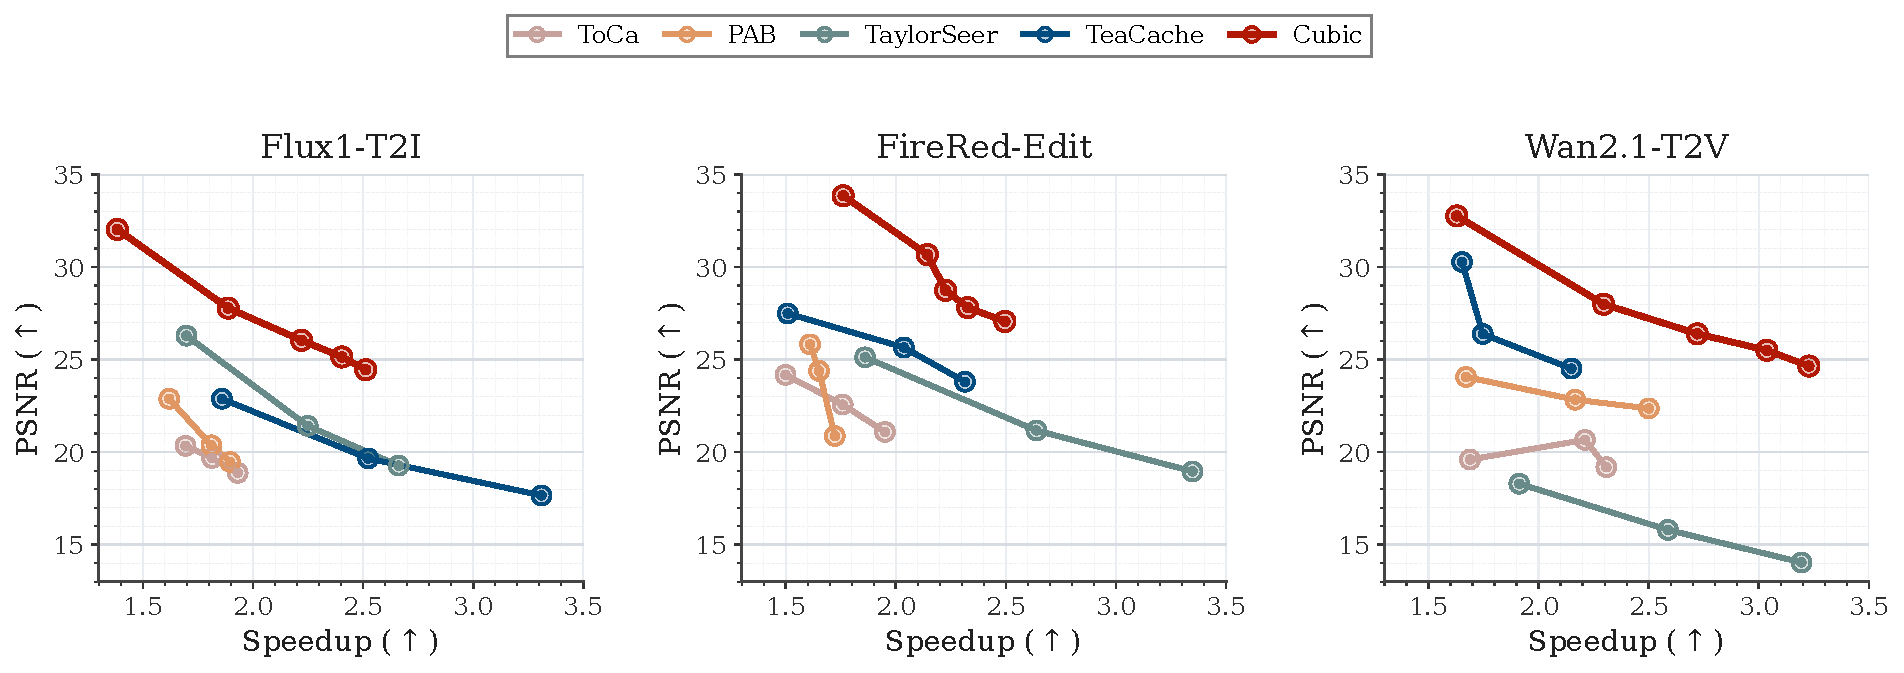
\includegraphics[width=\linewidth]{figure/tradeoff.pdf}
    \caption{\cubic consistently achieves Pareto-optimal quality–efficiency trade-offs across all three generation tasks.}
    \label{fig:tradeoff}
\end{figure}
\begin{abstract}
Flow Matching (FM) has emerged as the dominant paradigm for state-of-the-art image and video generation, yet its reliance on full attention over lengthy sequences incurs significant latency. While existing caching methods reduce redundant computations, they yield suboptimal performance, fundamentally constrained by inflexible spatial granularity and empirical, model-specific heuristics.

To bridge this gap, we ground the caching mechanism in the geometric properties of the FM velocity field. We theoretically establish that the \textbf{curvature} inherently dictates the coupling between trajectory fluctuation and computational requirements, thereby providing a rigorous metric to quantify caching staleness loss and automatically derive adaptive granularity and optimal update intervals.

Translating this theoretical insight into practical acceleration, we present \cubic, a train-free caching framework. It bypasses expensive curvature computations via a zero-overhead proxy signal that dynamically guides spatial partitioning and budget-constrained update scheduling. At the system level, a sparse forward engine translates these optimal policies into efficient runtime, ensuring that theoretical guarantees directly translate into actual FLOP savings and linear speedup. Being model-agnostic and virtually hyperparameter-free, \cubic consistently outperforms state-of-the-art caching baselines in quality at customizable acceleration ratios (averaging 2.5$\times$) across Wan2.1, Flux.1, and FireRed-Image-Edit.
\end{abstract}
\section{Introduction}
\label{sec:intro}

Flow Matching (FM)~\cite{flowmatching,rectifiedflow,meanflow} has emerged as the dominant paradigm for state-of-the-art image~\cite{flux,qwenimage}, video~\cite{wan,hunyuan} and multi-modal~\cite{firered,omnidit,hunyuanimage3} generation. 
By learning a neural velocity field to guide the transport path, FM achieves faster convergence and more stable training than traditional diffusion objectives~\cite{ddpm,ddim}.
To capture long-range dependencies across spatiotemporal tokens, these models universally adopt Diffusion Transformers (DiT)~\cite{dit} equipped with full attention. However, the escalating sequence lengths combined with the quadratic complexity of full-attention impose a prohibitive computational burden. For instance, nearly one NVIDIA A100 hour is required to generate a mere 5-second clip on HunyuanVideo~\cite{hunyuan}, severely hindering real-time and interactive deployment.

Traditional acceleration techniques -- such as distillation~\cite{distill1,distill2,distill3}, quantization~\cite{sageattention1,sageattention2,sageattention2+,sageattention3} and sparse kernels~\cite{sparsevideogen,sparsevideogen2} --- typically require architecture modifications or costly retraining. 
In contrast, caching-based methods~\cite{teacache,pab,tokencache,blockdance,meancache,jano} have emerged as a light-weight, train-free alternative. They exploit temporal redundancy across adjacent denoising steps to bypass redundant computations. 
However, existing caching paradigms are fundamentally hindered by two limitations that prevent them from achieving optimal speed-quality trade-offs:
\begin{itemize}
    \item {\textbf{The Granularity Dilemma:}} Coarse-grained caching ignores spatial heterogeneity, aggressively skipping computations and causing noticeable artifacts; whereas fine-grained caching introduces prohibitive runtime overhead through fragmented memory access. 
    \item {\textbf{Reliance on Empirical Tuning:}} Most methods depend on model-specific, hand-tuned update intervals that lack a principled optimization objective, offering no formal guarantees on quality preservation under fixed compute budgets. 
\end{itemize}

To overcome these limitations, we must recognize the true mathematical nature of caching during FM sampling: reusing velocity output for $\tau$ steps is equivalent to extending the effective local integration step size of the ODE solver by a factor of $\tau$. 

This reframing immediately points to the solution. The "granularity dilemma" is essentially a step-size allocation problem, while the "empirical tuning" issue stems from the lack of a variable to bound numerical error. Both are inherently governed by a single geometric property: the \textbf{curvature} of the velocity field. FM training inherently encourages straight trajectories for fast convergence, but deviations from this ideal manifest as high curvature, strictly mandating smaller steps to prevent numerical divergence. Conversely, low-curvature regions seamlessly tolerate aggressively enlarged steps. Therefore, curvature provides a theoretically grounded indicator for determining spatial granularity and characterizing staleness error, offering a bridge between empirical caching strategies and principled cache scheduling. 

However, translating the theory into practice encounters two immediate barriers (detailed in Sec.~\ref{sec:motiv_theory}): computing exact curvature requires prohibitive Jacobian operations, and the mathematical mapping from curvature to actual caching error remains undefined. 

Taking curvature as the unified theoretical knob, we propose \cubic, an FM acceleration framework specifically designed to bridge these theoretical barriers into practical speedups. 
\begin{itemize}
    \item \textbf{Bypassing the Jacobian Barrier:} \cubic introduces a lightweight online monitor that estimates curvature via \emph{endpoint prediction drift}, replacing expensive gradient computations with simple algebraic subtraction.
    \item \textbf{Closing the Error Gap:} \cubic derives a closed-form error bound that scales as $\kappa \tau^2$. Using Lagrangian optimization, it converts this bound into a budget-constrained interval allocation rule, providing a principled alternative to purely empirical threshold tuning.
    \item \textbf{Efficient Execution:} A sparse forward engine translates the proposed caching plans into highly efficient runtime via dynamic KV cache updating, ensuring mathematical guarantees directly translate into actual FLOP savings and good generation quality.
\end{itemize}

As shown in Fig.~\ref{fig:tradeoff}, experiments across diverse generation tasks---Flux.1~\cite{flux} for text-to-image, Wan2.1~\cite{wan} for text-to-video, and FireRed~\cite{firered} for image editing---demonstrate that \cubic consistently outperforms state-of-the-art caching baselines, delivering superior generation quality at any given computational budget.
\section{Related Work}
\paragraph{Flow Matching}
Superseding traditional noise-prediction diffusion models~\cite{ddpm, ddim}, \emph{Flow Matching} (FM)~\cite{flowmatching,rectifiedflow} learns a continuous-time velocity field to transport samples from a prior to the data distribution along simple probability paths.
A canonical example is the straight-line interpolation path:
$$
x_t = (1 - t)\, x_0 + t\, x_1, \quad t \in [0, 1]
$$
This formulation yields a smoother, mathematically tractable vector field, drastically reducing the ODE integration steps required for high-fidelity generation. FM now serves as the default backbone for state-of-the-art generative architectures~\cite{opensora2,flux,wan,hunyuan,sd3,firered}.


\paragraph{Cache-based Acceleration}
Cache-based methods offer a training-free, plug-and-play acceleration paradigm by reusing redundant intermediate features along the denoising trajectory. Existing works explore a vast spectrum of caching granularities: from coarse step-level~\cite{teacache,magcache,meancache,taylorseer} or layer-level skipping~\cite{blockdance,adnan2025foresightadaptivelayerreuse}, to fine-grained attention partial reuse~\cite{pab,deltadit,ditfastattn}, and down to the most granular token-level selective updates~\cite{tokencache,ras,jano}. However, navigating this design space is fundamentally hindered by the granularity dilemma and an over-reliance on empirical heuristics.

\paragraph{Optimized Samplers and Kernels}
Another paradigm focuses on modifying the solving process or computational operators. Algorithmically, distillation and reflow techniques~\cite{distill1,rectifiedflow} reduce integration steps by distilling generation trajectories into simpler paths. System-wise, quantized~\cite{sageattention1} or sparse attention kernels~\cite{sparsevideogen} are developed to mitigate the quadratic attention bottleneck in long sequences. Despite their effectiveness, these methods typically require auxiliary training data or architecture-specific modifications. Importantly, they are orthogonal to \cubic, allowing for potential cumulative speedups.

\section{Motivation}

% 不讲 complexity
% \subsection{Observation: Spatially Heterogeneous Computational Demands}
% During inference, Flow Matching models exhibit significant spatial heterogeneity in computational demands~\cite{jano}. Specifically, different spatial regions within a generated sample require vastly different amounts of computation, correlating tightly with their inherent visual complexity. For instance, simple, static regions (e.g., backgrounds) can reach satisfactory convergence with merely around 10 steps, whereas detail-rich, dynamically evolving subjects require the full trajectory of 50 steps. This intrinsic non-uniformity implies immense potential for content-aware selective computation. However, to truly harness this characteristic, a fundamental question remains: \emph{why does this complexity-computation correlation inherently exist?}

\begin{figure}
    \centering
    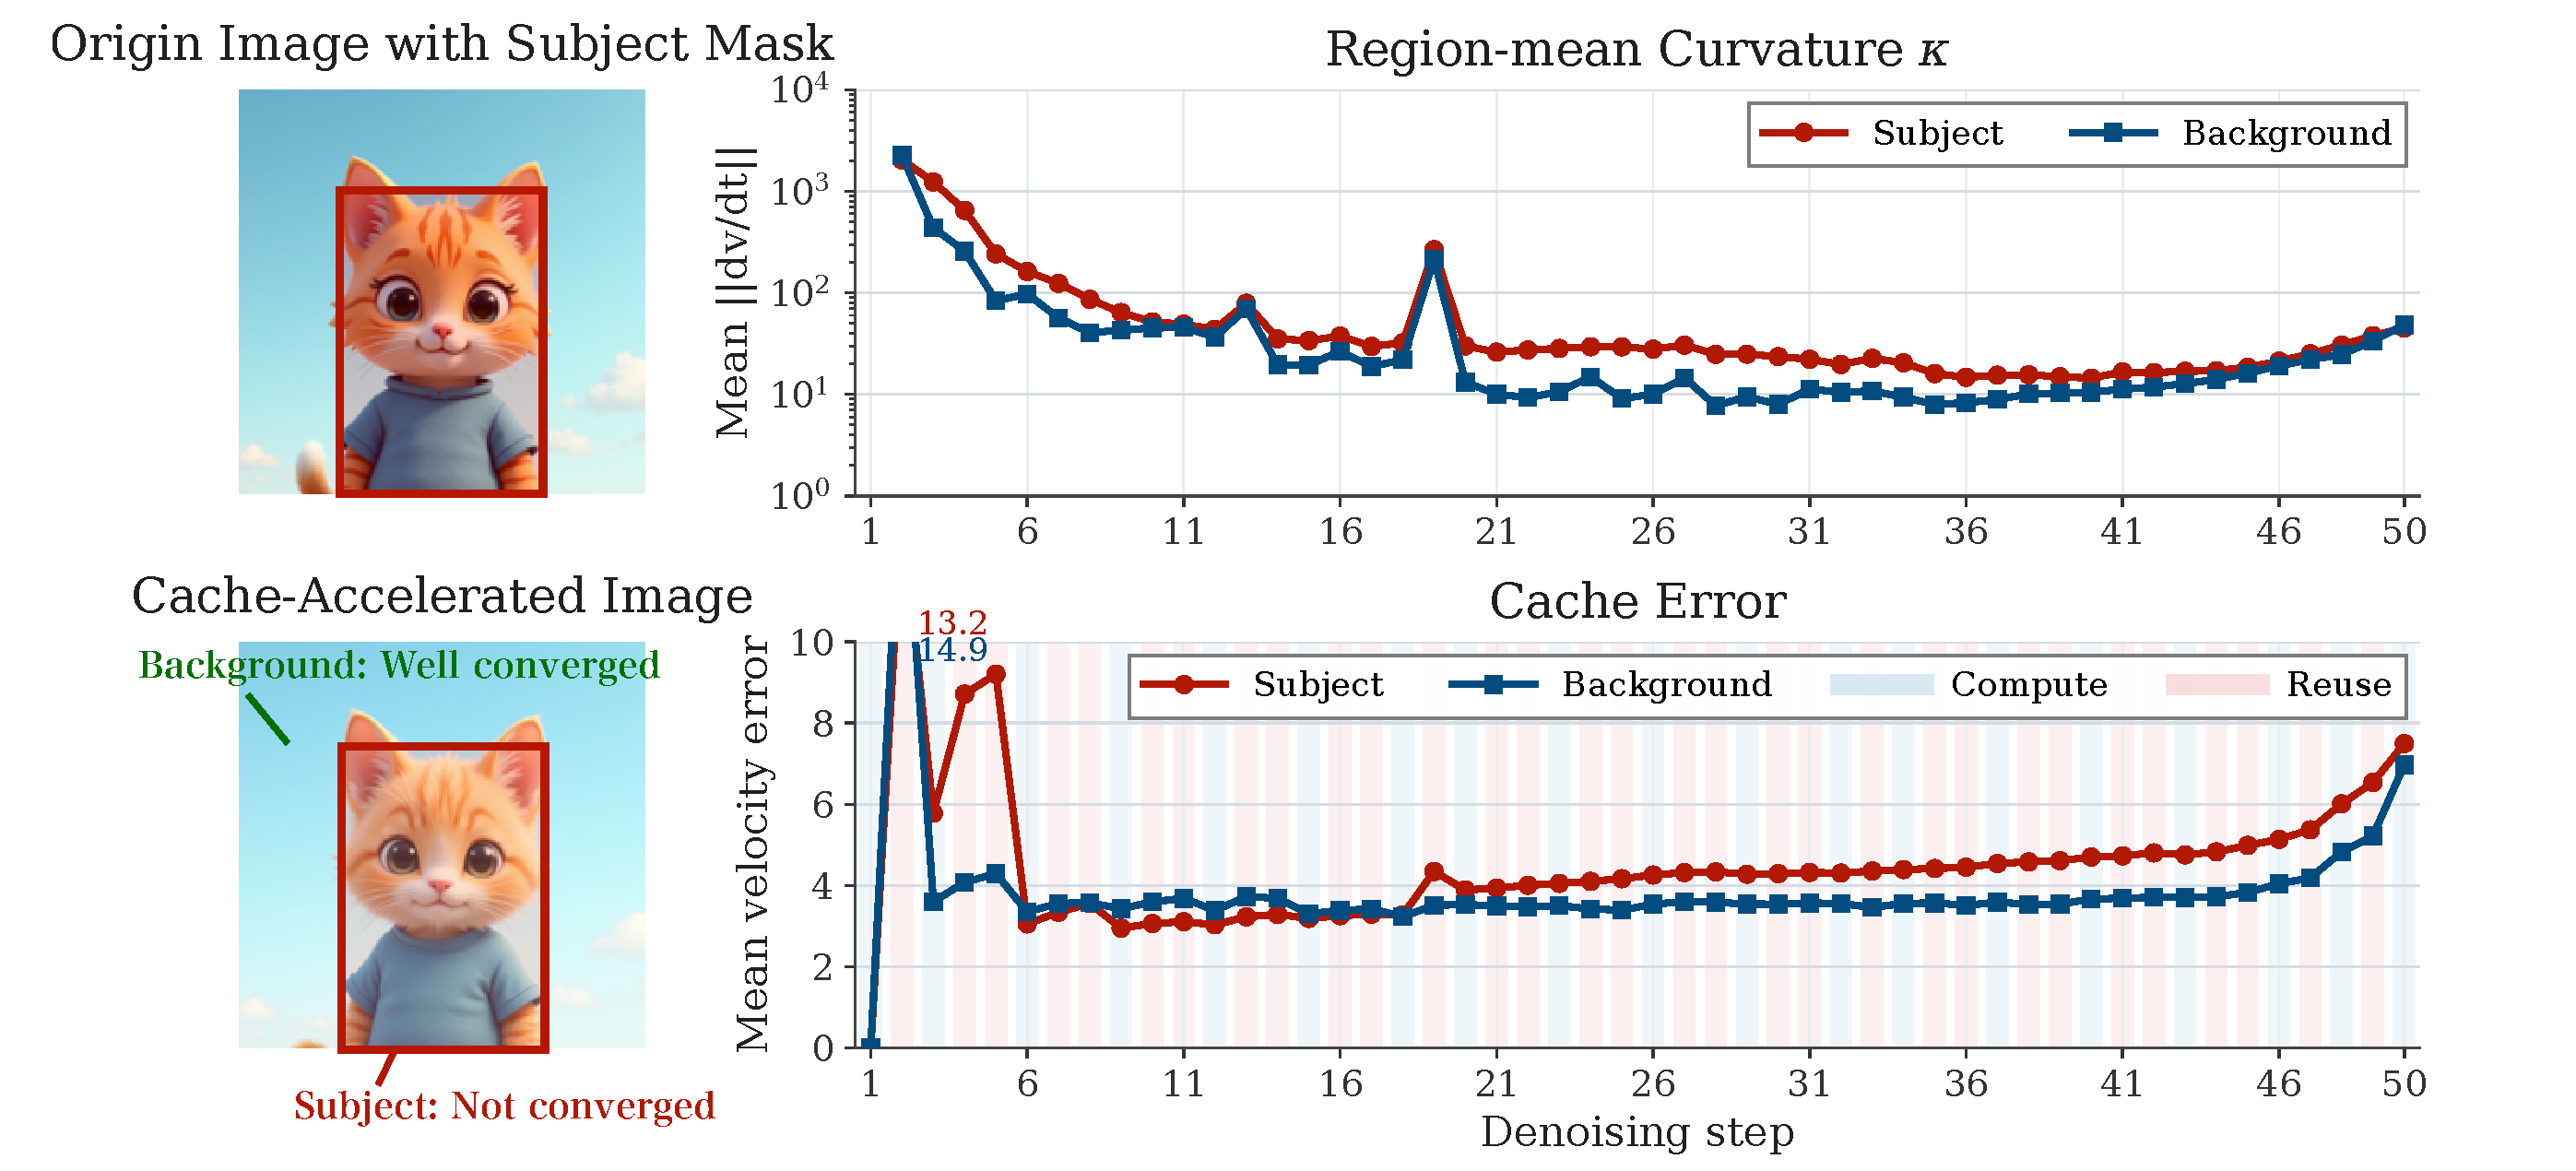
\includegraphics[width=\linewidth]{figure/motivation.pdf}
    \caption{Motivation Experiment: Subject regions exhibits higher curvature and incurs higher caching error accumulation.}
    \label{fig:motiv}
\end{figure}

\subsection{Observation: Spatially Heterogeneous Computational Demands}
During inference, Flow Matching models exhibit significant spatial heterogeneity in computational demands~\cite{jano}. Specifically, different spatial regions within a generated sample require vastly different amounts of computation to reach convergence. Usually, flat and static backgrounds converge faster than complex and dynamic subjects. This intrinsic non-uniformity implies immense potential for content-aware selective computation. However, to truly harness this characteristic, a fundamental question remains: \emph{what intrinsic property of the generation dynamics dictates these varying computational requirements?}

Fig.~\ref{fig:motiv} provides an empirical clue. Compared with the
background, the subject region shows higher trajectory curvature and accumulates
larger cache-induced velocity errors, indicating that trajectory curvature is
closely tied to region-wise cache tolerance.

\subsection{Theoretical Essence: Integration Step Size and Trajectory Curvature}
\label{sec:motiv_theory}
To understand why the cache-induced error in Fig.~\ref{fig:motiv}
varies across regions, we seek the answer from the Ordinary Differential Equation (ODE) perspective of Flow Matching. During inference, the continuous-time ODE is solved using a discrete time grid $0 = t_0 < t_1 < \cdots < t_K = 1$. Denoting the step size as $\Delta t = t_k - t_{k-1}$ (which can be uniform or non-uniform), the standard forward Euler iteration is formulated as:

\begin{equation}
    \label{wq:flow_matching_ode}
    x_{k+1} = x_k + \Delta t \cdot v_\theta(x_k, t_k).
\end{equation}
\begin{wrapfigure}{r}{0.5\columnwidth}
    % \vspace{-10pt}
    \centering
    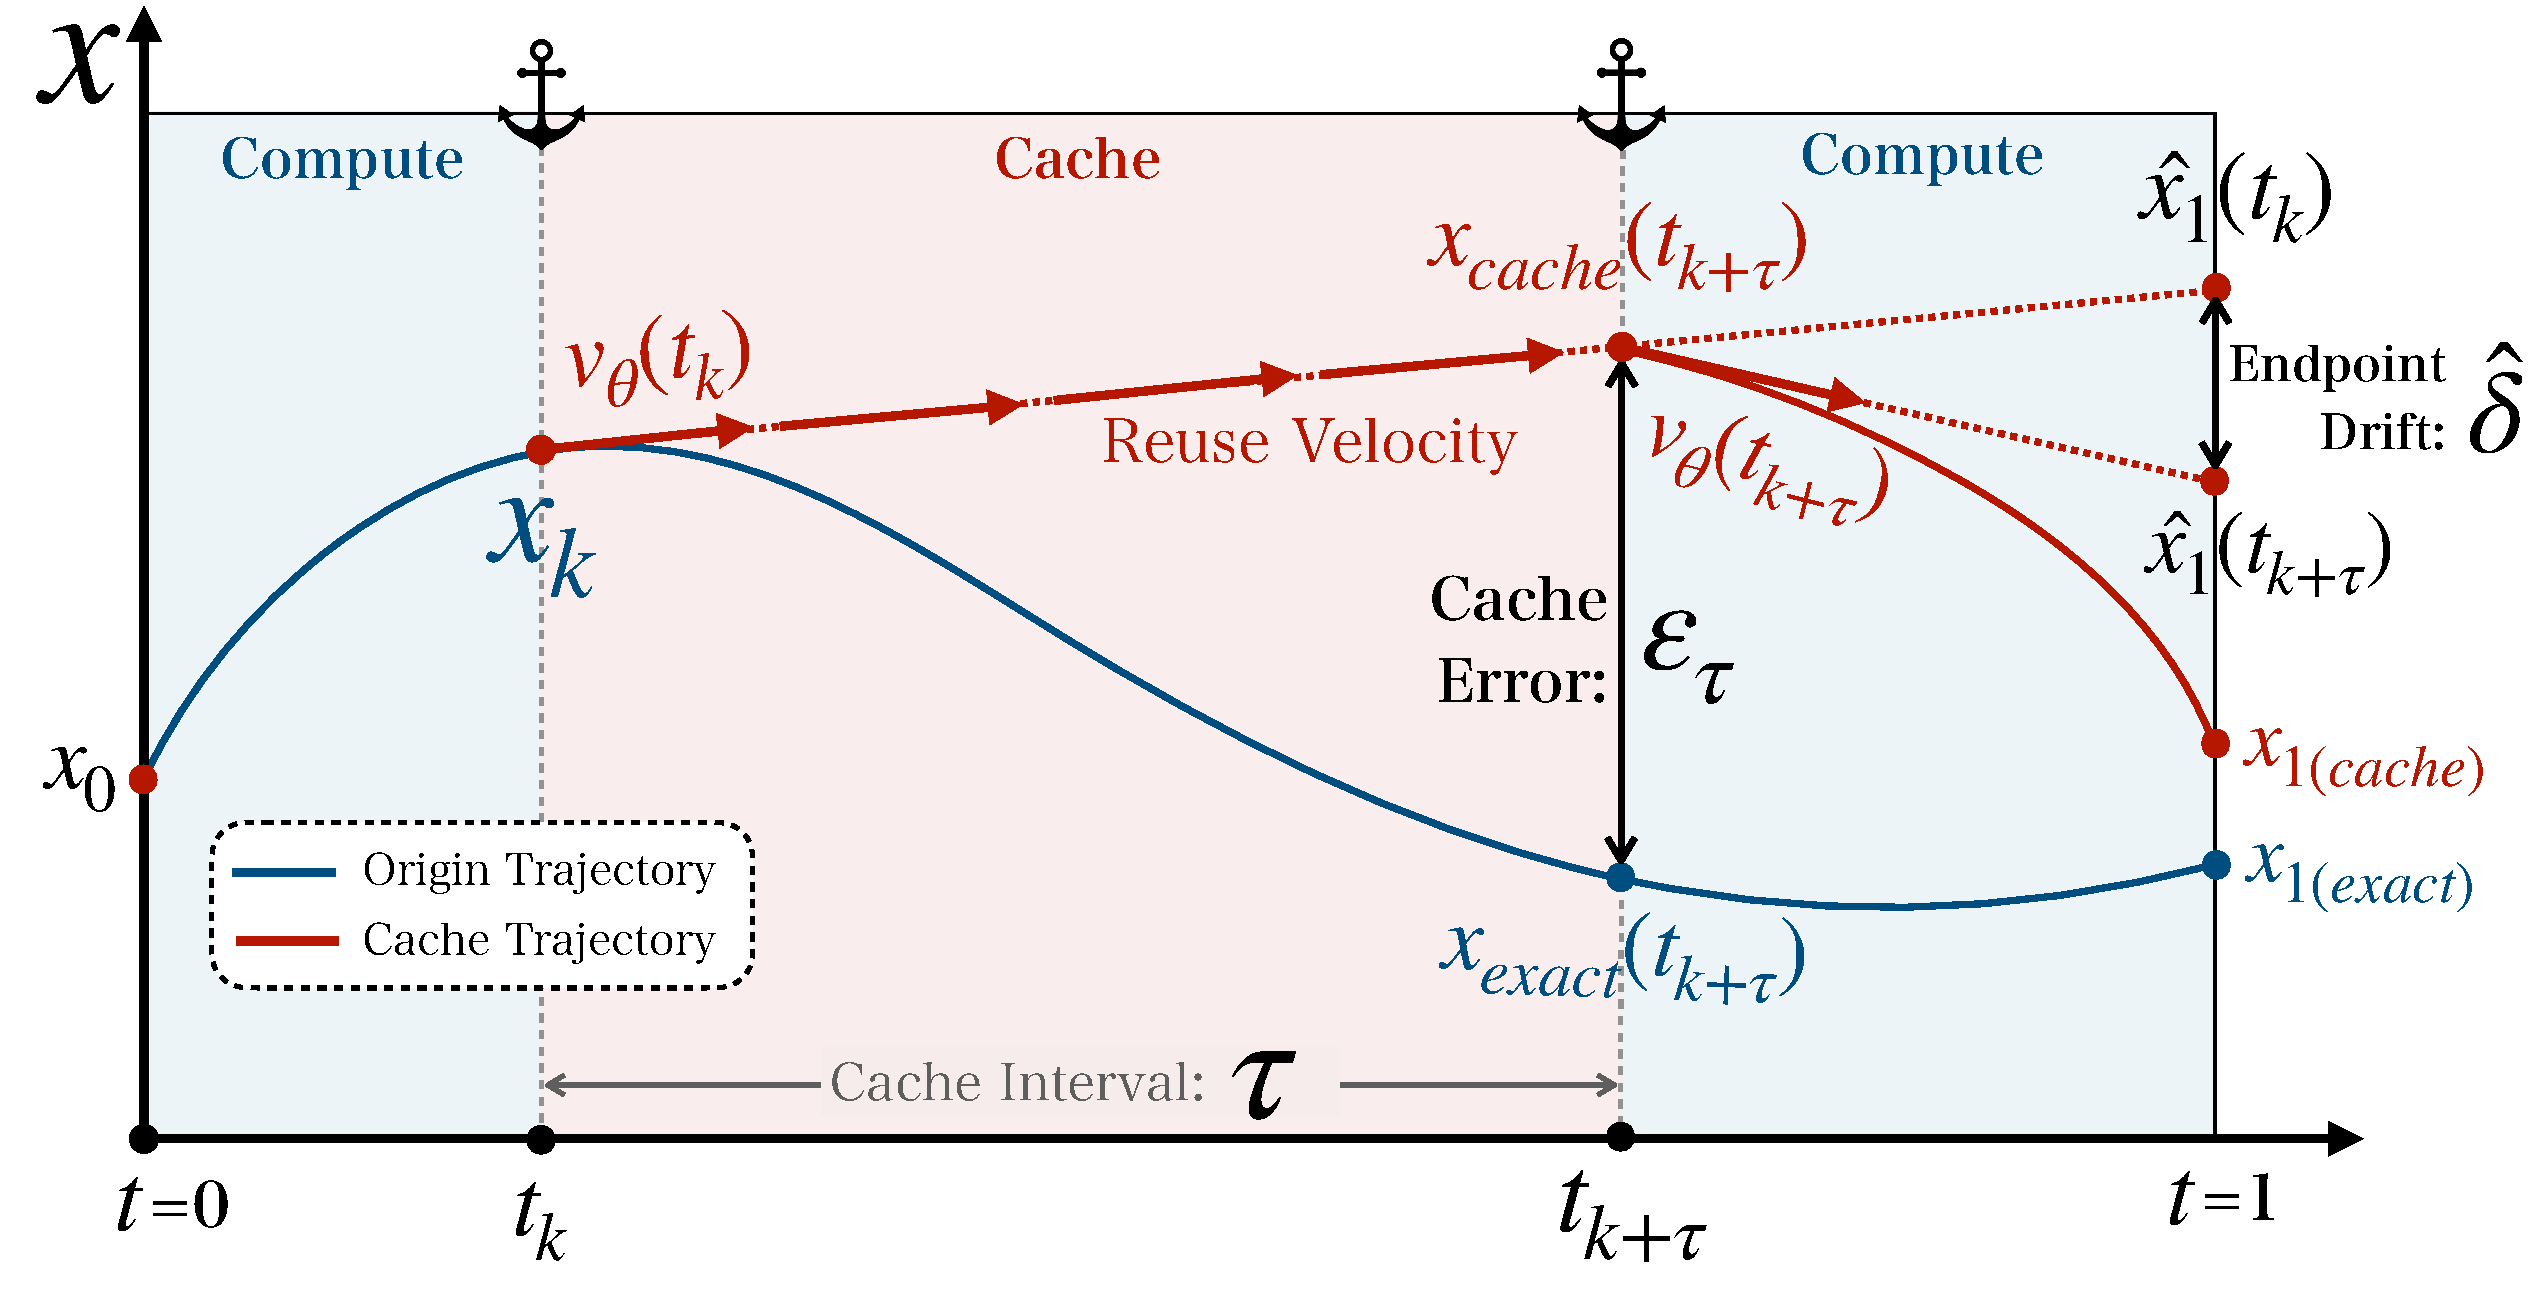
\includegraphics[width=\linewidth]{figure/method.pdf}
    \caption{Geometric interpretation of velocity reuse, cache error and endpoint drift in FM velocity field.}
    \label{fig:method}
   % \vspace{-8pt}
\end{wrapfigure}
As illustrated in Fig.~\ref{fig:method}, cache reuse can be interpreted as
holding the velocity prediction fixed over an extended interval. In other words,
reusing cached velocity features for multiple steps effectively enlarges the local
integration step size. We therefore conceptually reframe step
requirements across different regions as their
\emph{permissible integration step sizes}: fewer required updates imply that a
region can tolerate a larger effective $\Delta t$.

To achieve fast sampling, the FM training objective~\cite{rectifiedflow,meanflow}
inherently encourages the learned velocity field $v_\theta$ to be as constant as
possible along the temporal dimension, guiding the generation trajectory towards
a straight line, i.e., $dv_\theta / dt \equiv 0$. If the trajectory were perfectly
straight, a single large Euler step would solve the ODE exactly. In practice,
however, trajectories deviate from this ideal, and such deviation determines
whether enlarging effective step size is reliable.

We quantify this deviation as the \textbf{curvature} ($\kappa$) of the trajectory, mathematically captured by the material derivative of the velocity field along the flow:
\begin{equation}
    \label{eq:curvature}
    \kappa(t) = \frac{\partial v_\theta}{\partial t} + \left(\nabla_{x} v_\theta\right) \cdot v_\theta.
\end{equation}

High-curvature trajectories—driven by drastic velocity fluctuations—are highly sensitive to step size; aggressively enlarging the step introduces severe truncation errors that strictly mandate finer integration to prevent divergence. Conversely, low-curvature trajectories exhibit highly consistent velocities, where a single large step (more caching steps) is mathematically equivalent to multiple smaller ones.

\subsection{From Theory to Practice: The Practical Barriers}
While the theory dictates an optimal curvature-aware caching strategy, realizing it in practice encounters two immediate barriers. First, exact curvature is computationally forbidden. Obtaining $\kappa$ via Eq.~\ref{eq:curvature} requires computing the spatial Jacobian $\nabla_xV_\theta$ for massive sequences, introducing an overhead that completely defeats the purpose of caching. Second, the theoretical gap remains open. Even with a free oracle for $\kappa$, the exact mapping from ODE trajectory curvature to the actual feature-reuse "staleness error" is mathematically undefined. Without a closed-form error bound, any curvature-based design inevitably falls back into the trap of empirical tuning, lacking the formal guarantees needed for true optimality.
\section{Methodology}
\label{sec:method}

We present \cubic, a curvature-driven dynamic caching framework for FM generation. The core idea is to connect local trajectory geometry with runtime caching decisions: regions whose trajectories are locally straighter can tolerate more aggressive cache reuse, whereas regions with higher curvature should be refreshed more frequently. 


\subsection{Overview of the Inference Pipeline}
\label{sec:method_overview}

As illustrated in Fig.~\ref{fig:overview}, \cubic exploits the spatial heterogeneity of permissible step sizes by transforming the standard ODE solving process into an \emph{anchor-selective inference loop}. 

\begin{figure}[t]
    \centering
    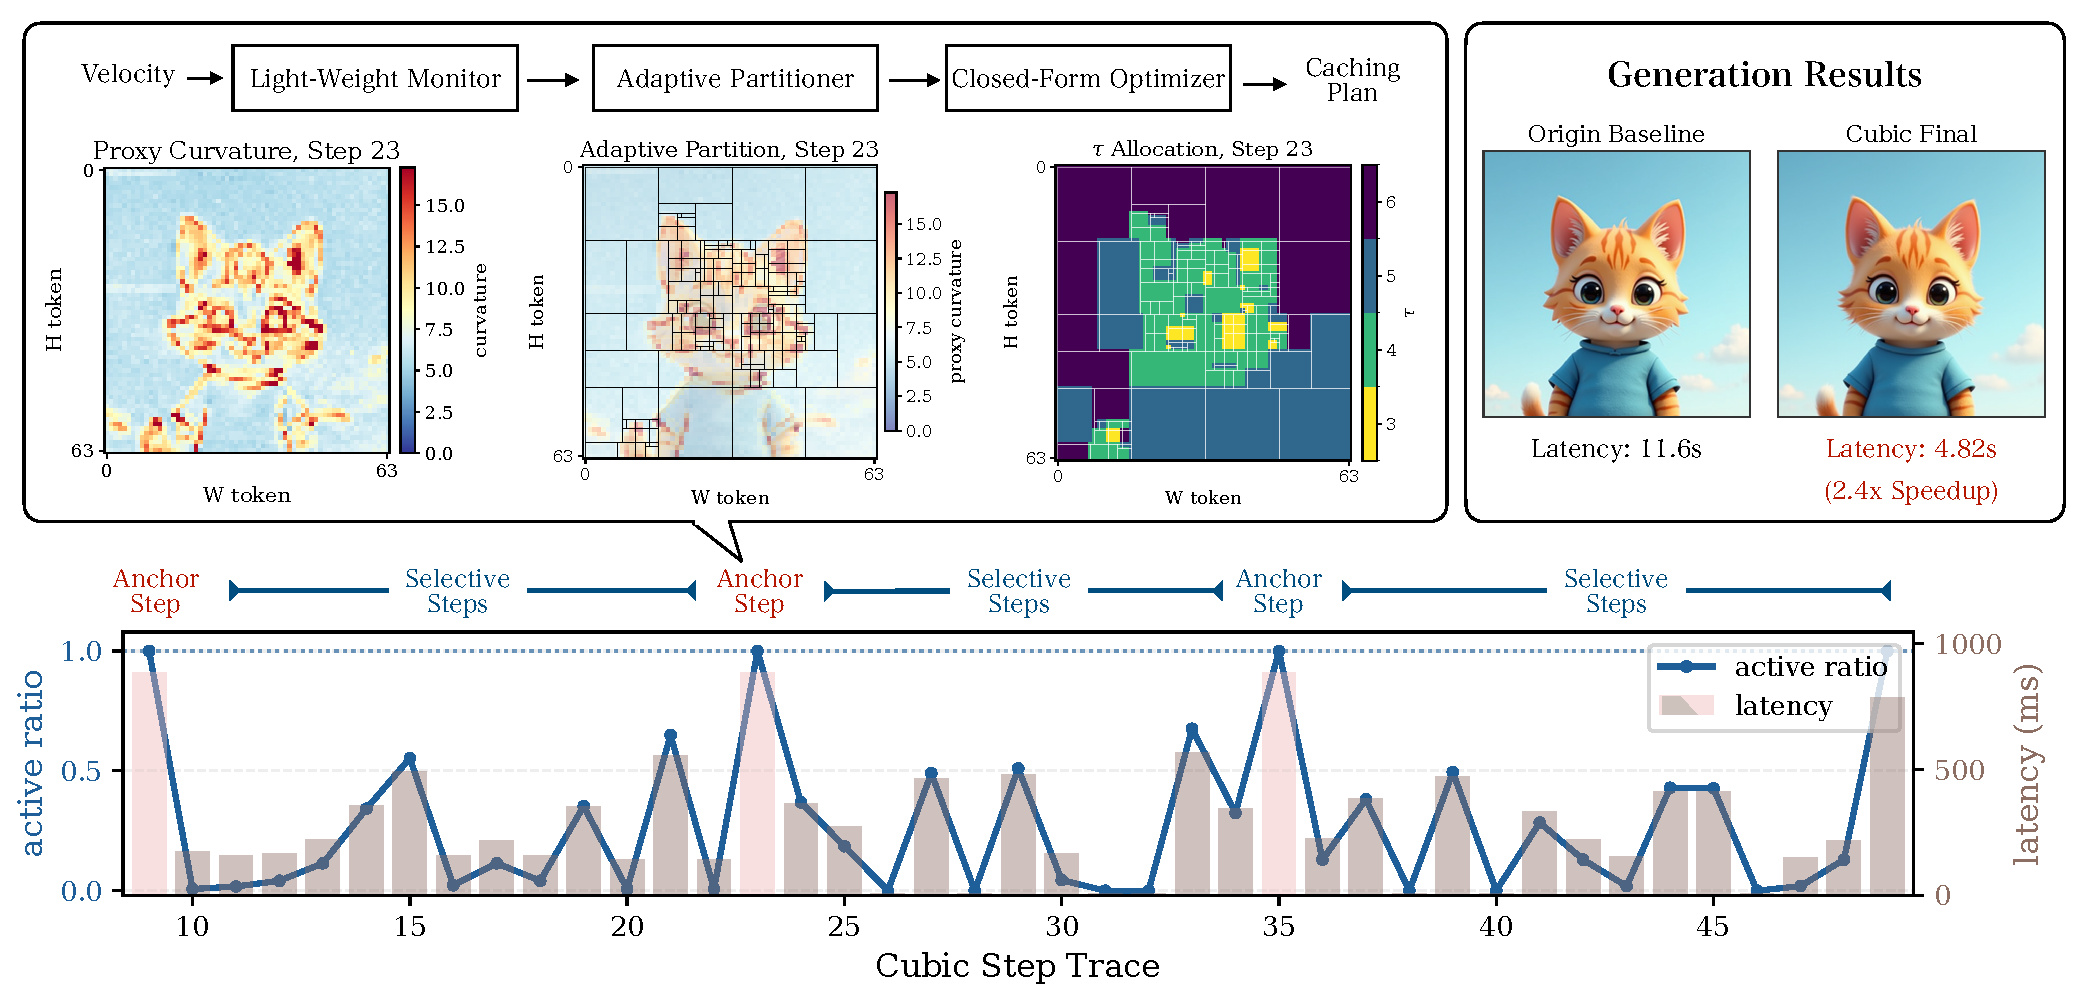
\includegraphics[width=\linewidth]{figure/overview.pdf}
    \caption{\cubic overview.}
    \label{fig:overview}
\end{figure}

The pipeline alternates between two types of steps:
\begin{itemize}
    \item \textbf{Anchor Steps:} Full forward passes that act as the ``brain'' of the system. They refresh the exact velocity prediction for all tokens, measure the geometric properties of the trajectory, and dynamically re-evaluate the caching policy.
    \item \textbf{Selective Steps:} Sparse forward passes that act as the ``muscle'' for acceleration. They compute only a dynamically chosen subset of tokens (active tokens), while the remaining tokens (frozen tokens) reuse cached intermediate states.
\end{itemize}
This anchor-selective decoupling divides the acceleration mechanism into two clean phases: \emph{estimation \& optimization} at anchor steps (Sec.~\ref{sec:anchor_step}), and \emph{sparse execution} at selective steps (Sec.~\ref{sec:selective_step}).
The two phases rest on different kinds of justification. The curvature proxy, the error model, and the budget-constrained interval allocation are derived from the ODE analysis in Appendix~\ref{app:cubic_theory}. The anchor horizon and the block partition are empirical system choices: they do not change the allocation rule, but select an operating point on the latency--quality frontier for a given architecture (Appendix~\ref{app:extra_exp}).
% This pipeline turns local trajectory geometry into a concrete execution policy: the monitor estimates curvature, the partitioner designs granularity, the optimizer assigns refresh intervals, and the runtime engine realizes those decisions as selective token computation.


\subsection{Anchor Steps: Estimation and Optimization}
\label{sec:anchor_step}

\paragraph{Curvature Estimation}
Directly computing local trajectory curvature is impractical at inference time because it requires Jacobian information which is expensive to compute. We therefore seek an online proxy that introduces light weight system cost. Our key observation is that if a token trajectory is locally straight, then its endpoint predicted by the current velocity field should remain nearly unchanged across successive observations. In contrast, trajectory curvature causes this endpoint prediction to drift.

For a spatial token indexed by $i$, we define its endpoint prediction at time $t$ as
\begin{equation}
    \hat{x}_1^{(i)}(t) = x^{(i)}(t) + (1 - t)\, v_\theta^{(i)}(x(t), t).
\end{equation}
Importantly, the monitor is updated only at anchor steps rather than at every sampler step. Let $\{t_{a_m}\}_{m=1}^{M}$ denote the anchor-step sequence. Interpreted in Fig.~\ref{fig:method}, we define the endpoint prediction drift between two consecutive anchor observations as
\begin{equation}
    \hat{\delta}^{(i,m)} = \hat{x}_1^{(i)}(t_{a_m}) - \hat{x}_1^{(i)}(t_{a_{m-1}}).
\end{equation}
As derived in Appendix~\ref{app:curvature_proxy}, to first order this drift scales proportionally to the local trajectory curvature $\kappa^{(i)}(t_{a_m})$, modulated by the remaining time horizon $(1-t_{a_m})$ and the step interval $\Delta t_{a_m} = |t_{a_m} - t_{a_{m-1}}|$.

Rearranging this relation directly gives the online curvature estimate:
\begin{equation}
    \hat{\kappa}^{(i)} = \left\|\hat{\delta}^{(i,m)}\right\|/\left[(1-t_{a_m})\,\Delta t_{a_m}\right].
\end{equation}

In practice, we compute this proxy in latent space and aggregate it to the token grid using the same patch granularity as the underlying DiT tokenizer, producing a token-space curvature map $\kappa \in \mathbb{R}^{F_t \times H_t \times W_t}.$ 

% \paragraph{Dynamic Spatial Partitioning}
% Assigning independent caching intervals to individual tokens incurs prohibitive scheduling overhead. Instead, \cubic groups adjacent tokens into rectangular blocks $\{B_b\}$ with shared update intervals. Crucially, to match the granularity to local trajectory complexity—fine blocks for curved regions, coarse blocks for straight regions—the partitioning must be spatially adaptive.

% Derived in Appendix~\ref{app:parition}, rather than relying on fixed grids, \cubic extracts a continuous geometric prior directly from the curvature map to guide the partitioning. We first isolate high-curvature "foreground" regions via thresholding and stabilize their boundaries. Using this prior, we then recursively bisect the token grid: foreground-dominated regions are assigned a finer target granularity, while background-dominated regions are assigned a coarser target. A region is split only if it exhibits mixed complexity (high intra-region variance) or exceeds its assigned target dimensions. 

% This yields adaptively-sized, strictly rectangular blocks that naturally conform to the underlying image geometry. Because this adaptive partitioning inherently isolates high-curvature outliers into dedicated finer blocks, we can safely represent each block's risk using a simple spatial mean:
% \begin{equation}
%     \kappa_b = \frac{1}{|B_b|} \sum_{i \in B_b} \hat{\kappa}^{(i)}.
% \end{equation}
% This block-wise curvature map $\{\kappa_b\}$ serves as the direct input for the subsequent budget-constrained interval optimization.

However, assigning independent caching intervals to individual tokens incurs prohibitive scheduling overhead. Instead, \cubic groups adjacent tokens into rectangular blocks $\{B_b\}$ that share a unified update interval. Sharing an interval also keeps neighboring tokens, which attend to each other with high attention weights in DiT self-attention, at the same cache age. Under per-token schedules, adjacent tokens would read keys and values computed at different steps (Sec.~\ref{sec:selective_step}), and this local inconsistency propagates through subsequent layers. To balance spatial granularity and scheduling efficiency, we employ a lightweight partitioning strategy guided by the curvature map (detailed in Appendix~\ref{app:parition}). Once the partition $\mathcal{P}=\{B_b\}$ is established, we aggregate the token-wise proxy into a representative block-wise score using a spatial mean:
    $\kappa_b = \frac{1}{|B_b|} \sum_{i \in B_b} \hat{\kappa}^{(i)}.$
This block-wise curvature map $\{\kappa_b\}$ serves as the direct input for the subsequent budget-constrained interval optimization.

\paragraph{Cache Error Modeling}
After obtaining a representative curvature for each block, \cubic determines how long each block may safely reuse cached outputs. Consider a block $b$ that is fully recomputed at an anchor step $t_0$, yielding the cached velocity $v_{\text{cache}}^{(b)} = v_\theta^{(b)}(x(t_0), t_0)$. If this block is frozen for the subsequent $\tau_b$ selective steps, the same cached velocity is continuously reused throughout the interval $[t_0, t_0+\tau_b \Delta t]$.

Let $x_{\text{exact}}^{(b)}(t)$ denote the exact trajectory, and $x_{\text{cache}}^{(b)}(t)$ denote the trajectory obtained by reusing the cached velocity. We define the cache-induced state truncation error at the end of the reuse window as:
\begin{equation}
    \varepsilon_{\tau_b}^{(b)} = x_{\text{cache}}^{(b)}(t_0 + \tau_b \Delta t) - x_{\text{exact}}^{(b)}(t_0 + \tau_b \Delta t).
    \label{eq:error_def}
\end{equation}
As derived in Appendix~\ref{app:error_modeling}, if the curvature is bounded within the reuse window, this accumulated error is bounded by the local trajectory curvature:
\begin{equation}
    \label{eq:error_bound}
    \left\|\varepsilon_{\tau_b}^{(b)}\right\|
    \lesssim
    \frac{1}{2}\,\kappa_b\,\tau_b^2\,\Delta t^2.
\end{equation}
This result directly exposes the desired behavior: blocks with low curvature can tolerate longer reuse intervals, while high-curvature blocks should be updated more often.

\paragraph{Update Interval Optimization} 
\label{sec:optimizer}

We formalize interval allocation as a budget-constrained optimization problem. Let $\rho$ denote the target speedup, $\tau_b$ the update interval for block $b$, and $|\mathcal{B}_b|$ its spatial size (i.e., number of tokens). Because the adaptive partitioner yields blocks of varying sizes, the optimization must be weighted by block size.

\begin{equation}
\min_{\tau_b \ge 1} \; \sum_{b=1}^{\mathcal{B}} |\mathcal{B}_b| \, \kappa_b^\alpha \tau_b^\beta
\quad \text{s.t.} \quad
\sum_{b=1}^{\mathcal{B}} \frac{|\mathcal{B}_b|}{N} \frac{1}{\tau_b} = \frac{1}{\rho},
\end{equation}
where $N = \sum_{b=1}^{\mathcal{B}} |\mathcal{B}_b|$ is the total number of tokens in the image, $\rho > 1$ is the target speedup factor, and $\tau_b \ge 1$ are the block-wise update intervals. The objective function minimizes the total expected squared error across the entire image, weighted by the number of tokens $|\mathcal{B}_b|$ per block, with the error bound per block squaring to $\kappa_b^\alpha \tau_b^\beta$. The constraint ensures that the token-weighted average update rate $\mathbb{E}[1/\tau_b]$ equals the reciprocal of the target speedup $1/\rho$, exactly enforcing the compute budget.
Note that $\rho$ specifies the compute budget of the selective steps only. Anchor steps and the full-compute steps at the beginning and end of sampling process all tokens. With $K_{\mathrm{full}}$ full-compute steps and $K_{\mathrm{sel}}$ selective steps, the overall token-compute fraction is $(K_{\mathrm{full}} + K_{\mathrm{sel}}/\rho)/(K_{\mathrm{full}} + K_{\mathrm{sel}})$, and the measured wall-clock speedup additionally reflects system overhead.
% To minimize the total expected squared error across the \emph{entire} image, the objective function is naturally weighted by the number of tokens in each block. By squaring the truncation error bound in Eq.~\ref{eq:error_bound}, we have:
% \begin{equation}
%     \min_{\tau_b \ge 1}\; \sum_{b=1}^{\mathcal{B}} |\mathcal{B}_b| \, \kappa_b^\alpha \tau_b^\beta.
% \end{equation}
% The compute budget constraint requires that the block-weighted average update rate strictly equals the reciprocal of the target speedup. Let $N = \sum_{b=1}^{B} |B_b|$ be the total number of tokens. The constraint is formulated as:
% \begin{equation}
%     \sum_{b=1}^{\mathcal{B}} \frac{|\mathcal{B}_b|}{N} \frac{1}{\tau_b} = \frac{1}{\rho}.
% \end{equation}
Intuitively, this ensures proportional FLOP savings: freezing a large block (high $|\mathcal{B}_b|$) for $\tau_b$ steps yields strictly greater computational reduction than freezing a smaller block with the same interval.

As derived in Appendix~\ref{app:optimal_interval} via the Lagrange multiplier method, the block size weights $|\mathcal{B}_b|$ appear on both the objective and the constraint. Consequently, they cancel out during the first-order optimality condition. The resulting optimum is $\tau_b^\star \propto \kappa_b^{-\gamma}$ with $\gamma=\alpha/(\beta+1)$, so the allocation depends on the two error exponents only through $\gamma$. Substituting the theoretical defaults $(\alpha,\beta)=(2,4)$ gives $\gamma=2/5$ and yields the final allocation rule:
% \begin{equation}
%     \tau_b^\star \propto \kappa_b^{-\alpha/(\beta+1)}.
% \end{equation}

\begin{equation}
    \tau_b^\star \propto \kappa_b^{-2/5}.
\end{equation}
Thus, \cubic naturally assigns shorter intervals to high-curvature blocks and longer intervals to low-curvature ones, irrespective of their spatial sizes. In implementation, the continuous solution is discretized to valid integer bounds. 

\paragraph{Effective ODE Strides}
To ensure optimized intervals translate into actual FLOP savings, anchor steps dictate a selective phase length of $2\tau_{\max}$, where $\tau_{\max} = \max_{b \in \mathcal{P}} \tau_b$. This receding-horizon rule is tied to the current allocation: it gives the blocks assigned the longest interval enough steps to execute their reuse schedule before curvature is re-estimated, so that caching operations serve as \emph{effective ODE strides} rather than being overwritten by the next anchor step. The factor of two is an empirical default rather than a theoretical optimum. If the curvature of a block changes within the window, its schedule is stale only until the next anchor step, which re-measures curvature and assigns shorter intervals to blocks whose curvature has increased. Appendix~\ref{app:anchor_ablation} compares this rule with shorter and longer horizons and with a fixed anchor gap.


\subsection{Selective Steps: Sparse DiT Execution}
\label{sec:selective_step}

% \paragraph{Anchor Step Trigger} The duration of the selective phase is dynamically determined to guarantee actual computational efficiency. Rather than using a fixed length, \cubic sets the selective phase length to $2\tau_{\max}$, where $\tau_{\max} = \max_{b \in \mathcal{P}} \tau_b$. This design ensures that even the block with the longest assigned interval completes at least one full cache reuse cycle before the global cache is refreshed at the next anchor step. Consequently, it prevents degenerate scheduling where anchor steps are triggered too frequently, which would otherwise nullify the FLOP savings of the selective phase.



\paragraph{Sparse Forward with KV Cache} Given the partition $\mathcal{P}$ and the block intervals $\{\tau_b\}$ at anchor step, the active blocks at selective step $k$ are defined as
\begin{equation}
    \mathcal{A}_k = \{ b \in \mathcal{P} \mid s_k \bmod \tau_b = 0 \},
\end{equation}
where $s_k$ is the local step index within the selective phase. The interval $\tau_b$ is an integer with $\tau_b \ge 1$. A block with $\tau_b = 1$ is recomputed at every selective step, and a block with $\tau_b > 1$ is recomputed every $\tau_b$ steps and stays frozen in between. This update-and-reuse cycle repeats until the next anchor step. The active blocks induce the active and frozen token sets
\begin{equation}
    \Omega_k^{\mathrm{act}} = \bigcup_{b \in \mathcal{A}_k} \mathcal{B}_b,
    \qquad
    \Omega_k^{\mathrm{frz}} = \Omega \setminus \Omega_k^{\mathrm{act}}.
\end{equation}

At each DiT layer, \cubic only computes the active tokens. To maintain full-sequence spatial dependencies without recomputing frozen tokens, the attention mechanism for active tokens queries against a reconstructed full sequence. Specifically, the newly computed Key/Value (KV) tensors for active tokens are concatenated with the cached KV tensors of frozen tokens to form the full KV states:
\begin{equation}
    K_\ell^{\mathrm{full}} = K_\ell^{\mathrm{act}} \oplus K_\ell^{\mathrm{frz}}, \quad
    V_\ell^{\mathrm{full}} = V_\ell^{\mathrm{act}} \oplus V_\ell^{\mathrm{frz}}.
\end{equation}
Attention is then evaluated as:
\begin{equation}
    Y_\ell^{\mathrm{act}} =
    \mathrm{Attn}\!\left(
    Q_\ell^{\mathrm{act}},
    K_\ell^{\mathrm{full}},
    V_\ell^{\mathrm{full}}
    \right).
\end{equation}
Crucially, after the attention computation, \cubic updates the cached KV entries for the active tokens in-place with the newly computed $K_\ell^{\mathrm{act}}$ and $V_\ell^{\mathrm{act}}$. This ensures that the per-layer KV cache progressively incorporates the latest cross-token interactions across successive steps, rather than remaining strictly static. The final output of the selective step is then formed by merging newly computed active-token outputs with cached frozen-token outputs.
% \begin{equation}
%     v_k(\Omega) =
%     \mathrm{Merge}\!\left(
%         v_k^{\mathrm{act}}(\Omega_k^{\mathrm{act}}),
%         v_{k-1,\mathrm{cache}}(\Omega_k^{\mathrm{frz}})
%     \right).
% \end{equation}

This selective forward engine is the component that actually yields computational savings: active tokens traverse the full DiT computation path, whereas frozen tokens participate only through cache reuse.


\section{Evaluation}
\subsection{Experiments Setup}
\paragraph{Models and Baselines.}
We evaluate \cubic across three representative generative settings: text-to-image generation using Flux-1-dev~\cite{flux}, instruction-guided image editing using FireRed-Image-Edit-1.0~\cite{firered}, and text-to-video generation using Wan2.1-T2V-1.3B~\cite{wan}. We compare with state-of-the-art feature caching baselines, including TokenCache (ToCa)~\cite{tokencache}, TeaCache~\cite{teacache}, Pyramid Attention Broadcast (PAB)~\cite{pab}, and TaylorSeer~\cite{taylorseer}. 

\paragraph{Metrics and Evaluation Datasets} We measure acceleration using the end-to-end latency under the default inference settings of each task. Generation quality is evaluated with PSNR, SSIM, LPIPS, and FID/FVD for both image and video outputs. For image generation, we additionally report HPSv3~\cite{HPSv3}, while video generation is further evaluated using VBench metrics. Experiments are conducted on t2i-diversity-eval~\cite{brack2025howtotrain}, PIE-Bench++~\cite{Pie_bench}, and VBench~\cite{vbench} for image generation, image editing, and video generation, respectively.

\paragraph{Implementation} 
\label{sec:Implementation}
Experiments run on NVIDIA H100 using PyTorch. \cubic acts as a non-intrusive wrapper, with all methods sharing identical prompts and seeds for fair comparison. For caching baselines, we use their official implementations on Flux and Wan; for FireRed, which lacks official baseline support, we implement compatible versions (details in Appendix.~\ref{app:detail_result}). Our full codebase will be open-sourced.

\subsection{Main Results: Pareto-Optimal Acceleration}
\paragraph{Quantitative Comparison}
% 可以看到，Cubic在加速比更高的同时，比起其他cache加速方法达到了更高的生成质量。值得注意的是，对于attention在计算中耗时更大的模型（wan2.1),cubic更容易实现更高的加速。
We evaluate the quality and efficiency of images and videos generated with \cubic (std: $\rho=2$, fast: $\rho=4$) against baseline methods, and summarize the results in Table \ref{tab:results}. Compared with existing caching-based acceleration methods, \cubic achieves higher speedups while preserving better generation quality. Notably, for models where attention accounts for a larger fraction of the overall computation, such as Wan2.1, \cubic can remove redundant computation more effectively, leading to more pronounced acceleration gains.
\begin{table*}[t]
\centering
\caption{Quantitative evaluation of inference efficiency and visual quality in generation models.}
\resizebox{\textwidth}{!}{
\begin{tabular}{l c c c c c c c c}
\toprule
\textbf{Model} & \textbf{Method} 
& $\mathrm{Latency(s)}\downarrow$ 
& $\mathrm{Speedup}\uparrow$
& $\mathrm{PSNR}\uparrow$ 
& $\mathrm{SSIM}\uparrow$ 
& $\mathrm{LPIPS}\downarrow$ 
& $\mathrm{FID/FVD}\downarrow$ 
& $\mathrm{HPSv3/VBench}\uparrow$ \\
\midrule

\multirow{7}{*}{\textbf{Flux-1}} 
& $\mathrm{Baseline}$ & $11.59\pm0.05$ & -- & -- & -- & -- & -- & 10.68 \\
& $\mathrm{PAB}$ & $6.40\pm0.11$ & 1.81$\times$ & 20.37 & 0.7702 & 0.2574 & 77.37 & 10.65 \\
& $\mathrm{TeaCache}$ & $6.24\pm0.08$ & 1.86$\times$ & 22.88 & 0.8514 & 0.1490 & 45.87 & 10.83 \\
& $\mathrm{ToCa}$ &$ 6.39\pm0.04$ & 1.81$\times$ & 19.68 & 0.7493 & 0.2726 & 70.76 & 10.62 \\ 
& $\mathrm{TaylorSeer}$ & $6.83\pm0.08$ & 1.70$\times$ & 26.29 & 0.8920 & 0.0994 & \textbf{26.80} & 10.82 \\
\rowcolor{lightbluerow}
& \cubic~(std) & $6.14\pm0.24$ & 1.89$\times$ & \textbf{27.78} & \textbf{0.8998} & \textbf{0.0946} & 27.81 & 10.87 \\
\rowcolor{lightbluerow}
& \cubic~(fast) & $\mathbf{4.82\pm0.21}$ & \textbf{2.40$\times$} & 25.14 & 0.8457 & 0.1730 & 47.32 & \textbf{10.97} \\

\midrule

\multirow{7}{*}{\textbf{FireRed}} 
& $\mathrm{Baseline}$ & $39.14\pm0.09$ & -- & -- & -- & -- & -- & 8.17 \\
& $\mathrm{PAB}$ & $23.70\pm0.17$ & 1.65$\times$ & 24.39 & 0.8888 & 0.0929 & 39.41 & 7.95 \\
& $\mathrm{TeaCache}$ & $16.91\pm0.26$ & 2.31$\times$ & 23.80 & 0.8955 & 0.0995 & 41.03 & 7.83 \\
& $\mathrm{ToCa}$ & $20.06\pm0.04$ & 1.95$\times$ & 21.09 & 0.7884 & 0.1779 & 67.25 & 7.18 \\
& $\mathrm{TaylorSeer}$ & $21.04\pm0.04$ & 1.86$\times$ & 25.12 & 0.9102 & 0.0837 & 33.70 & \textbf{8.07} \\
\rowcolor{lightbluerow}
& \cubic~(std) & $18.26\pm0.57$ & 2.14$\times$ & \textbf{30.67} & \textbf{0.9538} & \textbf{0.0468} & \textbf{18.55} & 8.00 \\
\rowcolor{lightbluerow}
& \cubic~(fast) & $\mathbf{16.83\pm0.42}$ & \textbf{2.33$\times$} & 27.81 & 0.9201 & 0.0907 & 32.18 & 7.90 \\

\midrule

\multirow{7}{*}{\textbf{Wan 2.1}} 
& $\mathrm{Baseline}$ & $101.54\pm2.40$ & -- & -- & -- & -- & -- & 79.90 \\
& $\mathrm{PAB}$ & $40.60\pm0.10$ & 2.50$\times$ & 22.36 & 0.8000 & 0.1670 & 57.78 & 78.41 \\
& $\mathrm{TeaCache}$ & $61.44\pm1.92$ & 1.65$\times$ & 30.27 & 0.9270 & 0.0454 & 11.72 & 79.79 \\
& $\mathrm{ToCa}$ & $44.00\pm2.26$ & 2.31$\times$ & 19.19 & 0.7383 & 0.2405 & 84.04 & 78.42 \\
& $\mathrm{TaylorSeer}$ & $39.24\pm2.56$ & 2.59$\times$ & 15.80 & 0.6410 & 0.3521 & 137.06 & 78.82 \\
\rowcolor{lightbluerow}
& \cubic~(std) & $62.35\pm2.77$ & 1.63$\times$ & \textbf{32.76} & \textbf{0.9481} & \textbf{0.0317} & \textbf{7.92} & 79.37 \\
\rowcolor{lightbluerow}
& \cubic~(fast) & $\mathbf{37.32\pm0.62}$ & \textbf{2.72$\times$} & 26.39 & 0.8740 & 0.0986 & 31.76 & \textbf{80.03} \\

\bottomrule
\end{tabular}
}
\label{tab:results}
\end{table*}
\vspace{-7pt}
\paragraph{Sensitivity Test on Quality-Latency Trade-off}
Fig.~\ref{fig:tradeoff} reports the PSNR--speedup trade-off of \cubic and the compared baselines across different models. 
Across a wide range of speedup ratios, \cubic consistently attains higher PSNR (with correspondingly stronger SSIM, LPIPS, and FID/FVD; see Appendix~\ref{app:detail_result}), thereby lying on the Pareto frontier of the quality--latency trade-off.


% 这些实验都在flux上面做就好
\subsection{Validating Theoretical Foundations}
\vspace{-7pt}
\paragraph{Accuracy of Curvature Estimation}
\begin{figure}[t]
    \centering
    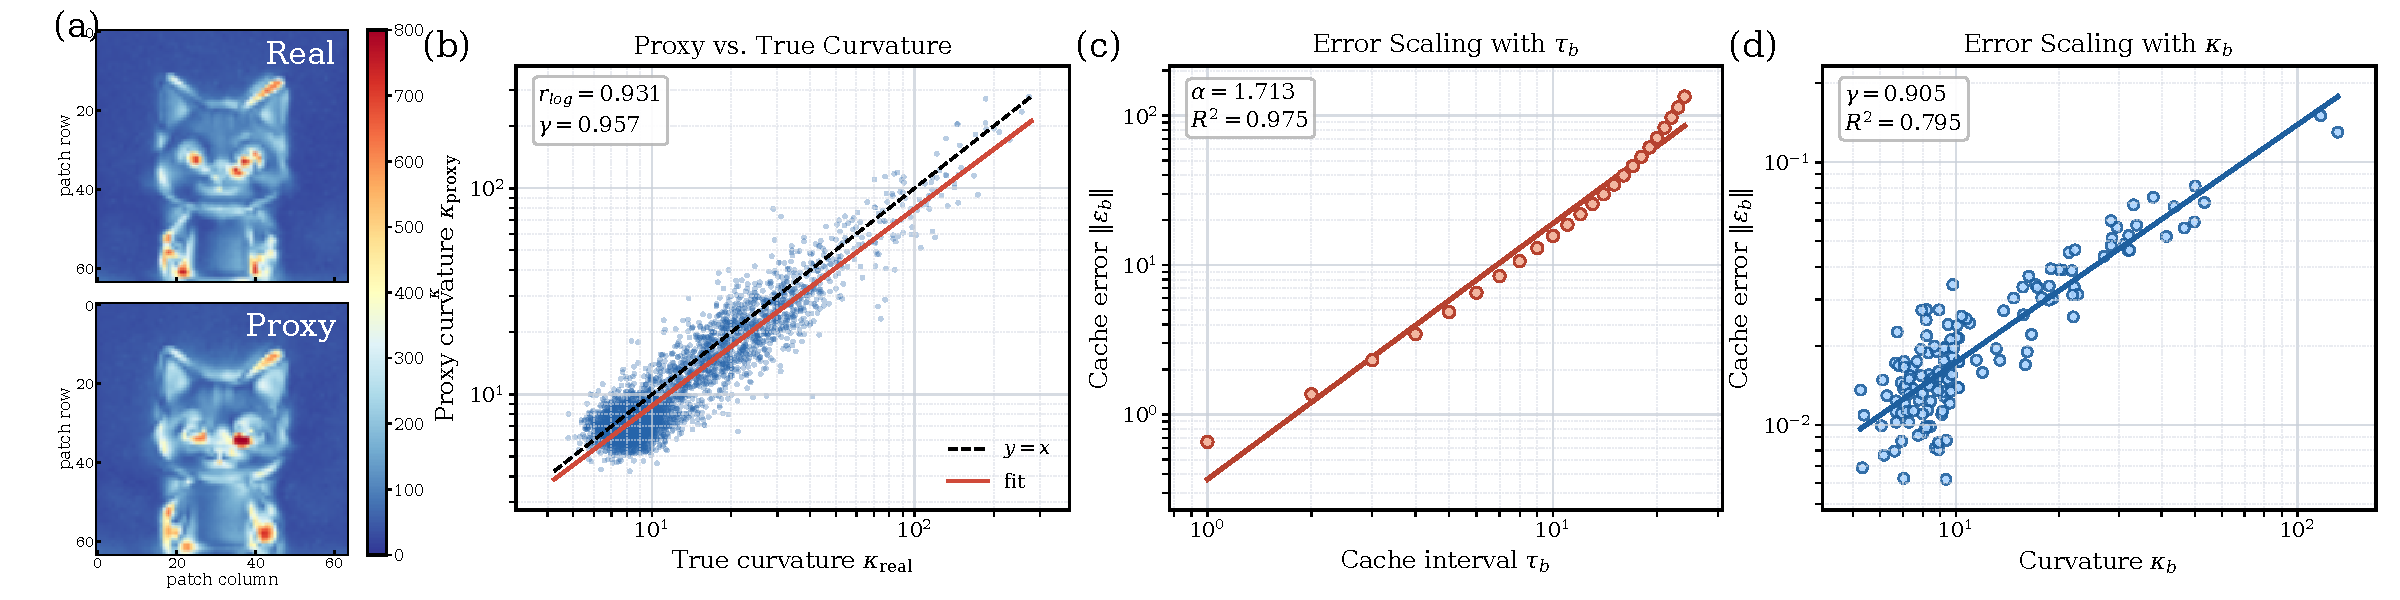
\includegraphics[width=\linewidth]{figure/theory.pdf}
    \caption{Validating the theoretical foundations of \cubic. (a) Visualization of real and proxy trajectory curvature on Flux. (b) Patch-wise correlation between $\kappa_{proxy}$ and $\kappa_{real}$. (c) Error scaling with reuse interval $\tau$. (d) Error scaling with curvature proxy $\kappa_b$.}
    \label{fig:theory_validation}
\end{figure}

We first validate whether the proposed endpoint-drift proxy accurately reflects true trajectory curvature. As shown in Fig.~\ref{fig:theory_validation}(a-b), the proxy closely matches both the spatial distribution and the relative magnitudes of the true curvature, exhibiting a strong linear correlation. This confirms that the proxy serves as a highly reliable online approximation for $\kappa^{(i)}$.

\vspace{-7pt}
\paragraph{Verification of the Cache Error Modeling}
We validate the cache-error bound derived in Eq.~\ref{eq:error_bound}. Fig.~\ref{fig:theory_validation}(c-d) confirm that the cache-induced error scales approximately quadratically with the reuse interval $\tau$ and linearly with the curvature proxy $\kappa$. These empirical scaling laws perfectly align with our theoretical derivations, demonstrating that the error model accurately captures the dominant behavior of cache-induced degradation.

% \paragraph{Optimality of Interval Allocation}
% % 相同speedup，验证-2/5次幂的tau分配生成效果是最好的。

\subsection{Ablation Studies on Core Components}

In Table.~\ref{tab:ablation}, we measure overhead and quality impact of \cubic components on Flux with standard setup.
\vspace{-7pt}
\paragraph{Monitor: Zero-Cost Proxy}
Despite introducing negligible system overhead, our drift proxy achieves generation quality remarkably close to that of the exact curvature computed via automatic differentiation. This validates our theoretical insight: the proxy successfully captures the essential trajectory geometry required for optimal scheduling, completely bypassing the prohibitive computational burden of explicit Jacobians.

\begin{wraptable}{r}{0.37\textwidth}
\vspace{-12pt}
\centering
\caption{Ablation Studies.}
\label{tab:ablation}
\footnotesize
\setlength{\tabcolsep}{3pt}
\renewcommand{\arraystretch}{0.95}
\begin{tabular}{@{}l c c c@{}}
\toprule
\textbf{Variant} & \textbf{Over.} & \textbf{FID}$\downarrow$ & \textbf{SSIM}$\uparrow$ \\
\midrule
\multicolumn{4}{l}{\footnotesize\itshape Monitor} \\
\quad Exact Jacobian & 603.9 & 33.1 & 0.967 \\
\rowcolor{lightbluerow}
\quad Proxy & \textbf{1.64} & 37.5 & 0.964 \\
\midrule
\multicolumn{4}{l}{\footnotesize\itshape Partitioner} \\
\quad Per-Token & 123.9 & 57.4 & 0.952 \\
\rowcolor{lightbluerow}
\quad Block-wise & \textbf{6.97} & \textbf{37.5} & \textbf{0.964} \\
\midrule
\multicolumn{4}{l}{\footnotesize\itshape Sparse Executor} \\
\quad w/o KV & 1.83 & 87.5 & 0.923 \\
\quad Static KV & 2.08 & 74.7 & 0.932 \\
\rowcolor{lightbluerow}
\quad Dynamic KV & 2.12 & \textbf{37.6} & \textbf{0.964} \\
\bottomrule
\end{tabular}
\vspace{-10pt}
\end{wraptable}


\vspace{-7pt}
\paragraph{Partitioner: Spatial Locality}
While per-token scheduling theoretically offers maximum flexibility, it incurs prohibitive indexing overhead. \cubic's block-wise strategy exploits the spatial locality inherent in DiT attention, drastically reducing scheduling complexity while maintaining contextual coherence, thereby achieving superior fidelity over the fine-grained baseline.
\vspace{-7pt}
\paragraph{Sparse Executor: Dynamic KV and Linear Scaling}
While a static KV cache prevents contextual isolation, it inevitably accumulates staleness errors. Our dynamic in-place update mechanism seamlessly resolves this by continuously refreshing the KV pool, minimizing staleness at negligible I/O cost.
Notably, layer-wise KV caches introduce memory requirements that scales with sequence length and layer count (e.g., 0.35GB for Flux vs. 17.68GB for Wan). To ensure deployability on memory-constrained hardware, we integrate asynchronous CPU offloading, which completely eliminates the GPU memory footprint of the cache at a marginal 5\% latency overhead.

\begin{wrapfigure}{r}{0.37\columnwidth}
\vspace{-10pt}
\centering
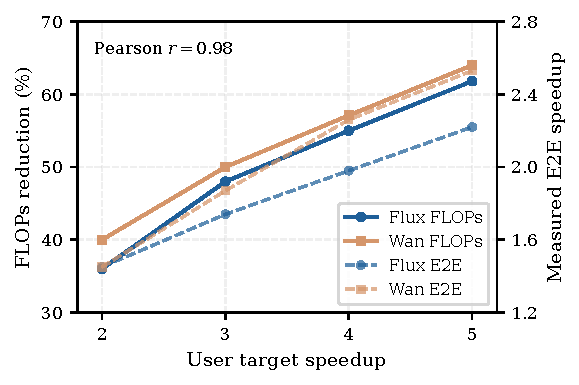
\includegraphics[width=\linewidth]{figure/flops.pdf}
\caption{FLOPs \& e2e speedup vs user-specified acceleration budget.}
\label{fig:flops}
\vspace{-10pt}
\end{wrapfigure}
Fig ~\ref{fig:flops} demonstrates that \cubic strategy effectively reduces flops in the selective phase, while the sparse executor efficiently transforms this into an end-to-end linear speedup. The speedup is lower than the user target because the speedup here only considers the selective phase; if end-to-end speedup is required, a simple conversion can be performed.



\subsection{Case Study: Components visualization}
\vspace{-7pt}
Due to space constraints, detailed visualizations of the dynamic pipeline are deferred to Appendix~\ref{app:case_study}. At a target speedup of $3\times$, \cubic executes five anchor steps. The scheduling exhibits a clear temporal evolution: early steps show high and heterogeneous curvature, leading to diverse interval allocations; middle steps capture localized high-curvature windows; and late steps converge to uniform curvature with consistent caching strategies. Throughout the process, the sparse ratio is stably maintained around $0.33$, and the step latency correlates strictly with the active ratio.
\section{Conclusion \& Limitation}
\label{sec:conclusion}
In this paper, we introduced \cubic, a training-free dynamic caching framework for efficient Flow Matching inference. By grounding the caching mechanism in the geometric properties of the velocity field—specifically, local trajectory curvature—\cubic adaptively partitions latents and optimizes update intervals to provably minimize error bounds. Comprehensive evaluations across diverse generation tasks demonstrate that \cubic establishes a superior quality-efficiency Pareto frontier compared to existing heuristic baselines. 
Nevertheless, our theoretical analysis is based on a forward-Euler abstraction of the sampling trajectory. While this offers a tractable link between curvature and cache-induced error, practical diffusion and flow-matching samplers often use multi-step, higher-order, or predictor--corrector updates, whose error constants and propagation patterns may differ. Therefore, our curvature-based scheduling rule should be viewed as a principled local approximation rather than a solver-agnostic guarantee, and extending the analysis to more general samplers is left for future work.

\section{Acknowledgements}
We would like to thank the anonymous reviewers for their insightful comments. This work is supported by the Fundamental and Interdisciplinary Disciplines Breakthrough Plan of the Ministry of Education of China (JYB2025XDXM910), NSFC for Distinguished Young Scholar under Grant 62225206, National Natural Science Foundation of China under Grants 62532006, 62495062, U23A600, and Beijing Natural Science Foundation under Grants L242017, L243001, L2603007. Jidong~Zhai is the corresponding author of this paper.



% We presented \cubic, a curvature-driven caching framework that translates ODE trajectory geometry into provably optimal cache scheduling for Flow Matching. Evaluations across diverse tasks confirm its superior quality-efficiency trade-offs over prior methods. Currently, the inherent memory overhead of layer-wise KV caches limits deployment on memory-constrained devices; future work will focus on frozen KV compression and efficient CPU offloading to mitigate this bottleneck.

\bibliographystyle{plain}
\bibliography{reference}
\newpage
\appendix
\appendix
\section{Theoretical Justification of \cubic}
\label{app:cubic_theory}

This section provides the theoretical justification for the curvature-aware
caching policy used in \cubic. We first analyze the state error induced by
cache reuse and show that it is jointly controlled by local trajectory
curvature and the cache reuse interval. We then convert this error model
into a block-wise interval allocation problem under a global computation
budget and derive the optimal reuse interval. Finally, we show how the
required curvature can be approximated online using endpoint prediction
drift without additional model forward passes.

\subsection{Curvature Approximation}
\label{app:curvature_proxy}

The optimal interval derived in Sec.~\ref{sec:optimizer} depends on the token-wise curvature $\kappa^{(i)}$. Directly computing $\kappa^{(i)}(t)=\|d v_\theta^{(i)}/dt\|_2$, however, requires Jacobian or higher-order derivative information and is therefore expensive for large-scale Flow Matching models. \cubic instead uses endpoint prediction drift as an online curvature proxy.

For a spatial token indexed by $i$, define the one-step endpoint prediction at time $t$ as
\begin{equation}
    \hat{x}_1^{(i)}(t)
    =
    x^{(i)}(t)
    +
    (1-t)
    v_\theta^{(i)}(x(t),t).
    \label{eq:app_endpoint_pred}
\end{equation}
This quantity is the endpoint that would be reached at $t=1$ if the current velocity were kept constant. If the local trajectory is nearly linear, endpoint predictions at nearby times should remain almost unchanged. In contrast, a curved trajectory produces a noticeable endpoint drift.

Taking the total derivative of Eq.~\eqref{eq:app_endpoint_pred} along the exact trajectory gives
\begin{align}
    \frac{d \hat{x}_1^{(i)}}{dt}
    &=
    \frac{d x^{(i)}}{dt}
    -
    v_\theta^{(i)}(x(t),t)
    +
    (1-t)
    \frac{d v_\theta^{(i)}}{dt}
    \nonumber \\
    &=
    (1-t)
    \frac{d v_\theta^{(i)}}{dt}.
    \label{eq:app_endpoint_derivative}
\end{align}
Let $t_{a_{m-1}}$ and $t_{a_m}$ be two consecutive anchor steps, and denote $\Delta t_{a_m}=t_{a_m}-t_{a_{m-1}}$. A first-order Taylor expansion gives
\begin{equation}
    \hat{\delta}^{(i,m)}
    =
    \hat{x}_1^{(i)}(t_{a_m})
    -
    \hat{x}_1^{(i)}(t_{a_{m-1}})
    \approx
    (1-t_{a_m})
    \frac{d v_\theta^{(i)}}{dt}(t_{a_m})
    \Delta t_{a_m}.
\end{equation}
Taking norms yields
\begin{equation}
    \left\|
    \hat{\delta}^{(i,m)}
    \right\|_2
    \approx
    (1-t_{a_m})
    \Delta t_{a_m}
    \kappa^{(i)}(t_{a_m}).
    \label{eq:app_drift_curvature_relation}
\end{equation}
Therefore, the normalized endpoint drift
\begin{equation}
    \hat{\kappa}^{(i)}
    =
    \frac{
    \left\|
    \hat{\delta}^{(i,m)}
    \right\|_2
    }{
    (1-t_{a_m})\Delta t_{a_m}
    }
    \label{eq:app_kappa_estimator}
\end{equation}
serves as an online approximation of $\kappa^{(i)}(t_{a_m})$.

This proxy uses only quantities already available at anchor steps, namely the current latent state and the model-predicted velocity. It therefore requires no additional model forward passes. 





\subsection{Error Modeling of Cache Reuse}
\label{app:error_modeling}

We first derive the local state error induced by cache reuse at the
position level. Consider a block $b$ that is fully recomputed at time
$t_0$, producing the cached velocity
\begin{equation}
    v_0^{(b)} = v_\theta^{(b)}(x(t_0),t_0).
\end{equation}
If this velocity is reused for the next $\tau_b$ solver steps, the local
approximate dynamics follow a zero-order hold:
\begin{equation}
    \frac{dx_{\textrm{exact}}^{(b)}(t)}{dt}=v_0^{(b)}.
\end{equation}
Let $x_{\textrm{exact}}^{(b)}(t)$ denote the exact trajectory. The cache-induced state
error is
\begin{equation}
    \varepsilon_b(t)
    =
   x_{\textrm{cache}}^{(b)}(t)-x_{\textrm{exact}}^{(b)}(t)
    =
    \int_{t_0}^{t}
    \left[
    v_0^{(b)}-v_\theta^{(b)}(x(t'),t')
    \right]dt'.
\end{equation}

We quantify the local trajectory curvature at block $b$ by the rate of
change of the velocity field along the exact trajectory:
\begin{equation}
    \kappa_b(t)
    =
    \left\|
    \frac{d v_\theta^{(b)}}{dt}(x(t),t)
    \right\|_2 .
    \label{eq:app_curvature_def}
\end{equation}
Assume that $\kappa_b(t)\le \bar{\kappa}_b$ within the reuse window. Then
the velocity mismatch satisfies
\begin{equation}
    \left\|
    v_0^{(b)}-v_\theta^{(b)}(x(t),t)
    \right\|_2
    \le
    \bar{\kappa}_b(t-t_0).
\end{equation}
Integrating over a reuse window of length $\tau_b\Delta t$ gives
\begin{equation}
    \left\|\varepsilon_b(t_0+\tau_b\Delta t)\right\|_2
    \le
    \frac{1}{2}
    \bar{\kappa}_b
    \tau_b^2
    \Delta t^2 .
    \label{eq:app_zoh_error_bound}
\end{equation}


The measured cache-induced error follows an approximate power-law dependence on both the reuse interval $\tau$ and the local curvature proxy $\kappa$, supporting the error bound in Eq.~\eqref{eq:app_zoh_error_bound}.

Therefore, cache reuse introduces a state error that grows linearly with
local curvature and quadratically with the reuse interval. Taking the
squared norm as the cache-loss surrogate gives
\begin{equation}
    \ell_b(\tau_b)
    =
     \left\|\varepsilon_b(t_0+\tau_b\Delta t)\right\|_2^2
    \lesssim
    \frac{1}{4}
    \bar{\kappa}_b^2
    \tau_b^4
    \Delta t^4 .
\end{equation}
Dropping shared constants yields the default surrogate
\begin{equation}
    \ell_b(\tau_b)
    \propto
    \kappa_b^2 \tau_b^4 .
    \label{eq:app_surrogate_default}
\end{equation}
More generally, we write
\begin{equation}
    \ell_b(\tau_b)
    =
    a_b
    \kappa_b^\alpha
    \tau_b^\beta ,
    \label{eq:app_general_surrogate}
\end{equation}
where the theoretical default is $(\alpha,\beta)=(2,4)$.
\subsection{Optimal Cache Reuse Interval under a Target Speedup}
\label{app:optimal_interval}

We next derive the optimal block-wise reuse interval under a target
speedup. Let $\tau_b$ denote the update interval of block $b$, and let
$\mathcal{B}_b$ be the set of  tokens contained in this block.
Since different blocks may contain different numbers of tokens, both the
cache-induced error and the computation reduction should be weighted by
the block size $|\mathcal{B}_b|$.

Using the generalized cache-loss surrogate from
Eq.~\eqref{eq:app_general_surrogate}, we consider the following
block-weighted optimization problem:
\begin{equation}
    \min_{\{\tau_b\}_{b=1}^{B}}
    \sum_{b=1}^{B}
    |\mathcal{B}_b|
    \kappa_b^\alpha
    \tau_b^\beta,
    \qquad
    \mathrm{s.t.}
    \quad
    \sum_{b=1}^{B}
    \frac{|\mathcal{B}_b|}{N}
    \frac{1}{\tau_b}
    =
    \frac{1}{\rho},
    \quad
    \tau_b\ge 1,
    \label{eq:app_interval_opt}
\end{equation}
where $N=\sum_{b=1}^{B}|\mathcal{B}_b|$ is the total number of spatial
tokens, $\rho$ is the target speedup, and $\kappa_b$ is the block-wise
curvature estimate. The constraint states that the block-size-weighted
average update rate equals the reciprocal of the target speedup.

Ignoring integer and box constraints, the Lagrangian is
\begin{equation}
    \mathcal{L}
    =
    \sum_{b=1}^{B}
    |\mathcal{B}_b|
    \kappa_b^\alpha
    \tau_b^\beta
    +
    \lambda
    \left(
    \sum_{b=1}^{B}
    \frac{|\mathcal{B}_b|}{N}
    \frac{1}{\tau_b}
    -
    \frac{1}{\rho}
    \right).
\end{equation}
Setting $\partial\mathcal{L}/\partial\tau_b=0$ gives
\begin{equation}
    |\mathcal{B}_b|
    \beta
    \kappa_b^\alpha
    \tau_b^{\beta-1}
    -
    \lambda
    \frac{|\mathcal{B}_b|}{N}
    \tau_b^{-2}
    =
    0.
\end{equation}
The block size $|\mathcal{B}_b|$ appears in both the objective and the
constraint, and therefore cancels out in the first-order optimality
condition. We obtain
\begin{equation}
    \tau_b^\star
    \propto
    \kappa_b^{-\alpha/(\beta+1)}.
    \label{eq:app_tau_general}
\end{equation}
With the squared-error default $(\alpha,\beta)=(2,4)$, this becomes
\begin{equation}
    \tau_b^\star
    \propto
    \kappa_b^{-2/5}.
    \label{eq:app_tau_two_fifths}
\end{equation}
Thus, high-curvature blocks are refreshed more frequently, whereas
low-curvature blocks can safely reuse cached states for longer intervals.

To satisfy the target speedup constraint, we normalize the proportional
rule. Let $\gamma=\alpha/(\beta+1)$. Then the continuous interval is
\begin{equation}
    \tilde{\tau}_b
    =
    \rho
    \cdot
    \frac{
    \frac{1}{N}
    \sum_{j=1}^{B}
    |\mathcal{B}_j|
    \kappa_j^\gamma
    }{
    \kappa_b^\gamma
    }.
    \label{eq:app_tau_closed_form}
\end{equation}
In practice, we use the squared-error default $\gamma=2/5$ and discretize
the interval as
\begin{equation}
    \tau_b
    =
    \mathrm{round}
    \left(
    \rho'
    \cdot
    \frac{
    \frac{1}{N}
    \sum_{j=1}^{B}
    |\mathcal{B}_j|
    \kappa_j^{2/5}
    }{
    \kappa_b^{2/5}+\varepsilon
    }
    \right),
    \label{eq:app_tau_discrete}
\end{equation}
where $\rho'$ absorbs the adjustment caused by rounding and clipping, and
$\varepsilon$ prevents numerical instability for near-zero curvature. We
set $\tau_{\min}=1$ so that high-curvature blocks can be recomputed at
every step.




% \subsection{Assumptions and Scope}\todo{}
% \label{app:assumptions}

% The above derivation relies on the following assumptions.

% \paragraph{Smoothness and bounded curvature.}
% Within each cache reuse window, the velocity field is assumed to be
% sufficiently smooth along the sampling trajectory, and the local curvature
% is assumed to be bounded. This ensures the quadratic time scaling of the
% ZOH error and justifies endpoint drift as a first-order curvature proxy.

% \paragraph{Mid-stage curvature stationarity.}
% \cubic mainly applies adaptive caching in the middle stage of sampling.
% At this stage, the global structure is typically established, while final
% high-frequency refinement has not yet dominated the dynamics. Therefore,
% curvature estimates from anchor steps can guide cache reuse over short
% subsequent windows.

% \paragraph{Approximate block-wise error additivity.}
% The optimization objective treats cache errors from different blocks as
% approximately additive. This is not exact for DiT backbones with global
% self-attention. However, \cubic periodically refreshes all token states at
% anchor steps, and during selective steps active tokens still attend to
% the full sequence through cached key/value states. Thus, cross-block error
% propagation is restricted within short reuse windows.

% \paragraph{Numerical stability near the endpoint.}
% Since the curvature proxy contains the normalization factor $(1-t)$,
% the estimate can become unstable near $t=1$. Therefore, \cubic restores
% full forward passes in the final sampling stage and uses $\varepsilon$ or
% stops updating the curvature proxy to avoid unstable scheduling decisions.

\section{Details of Partitioning Strategy}
\label{app:parition}

In Sec.~\ref{sec:anchor_step}, we introduced the morphology-guided adaptive partitioning strategy. We find that the exact partitioning scheme has a minor impact on overall performance. For long-sequence, high-overhead models such as Wan (sequence length 32760), we adopt morphology-guided partitioning to accurately select tokens; for shorter, fast-inference models (sequence length 4096), a simple fixed-size partitioning achieves comparable results with lower overhead. We provide the detailed algorithmic steps of the morphology-guided strategy here. The input is the raw token-space curvature map $\kappa \in \mathbb{R}^{F_t \times H_t \times W_t}$ computed at the current anchor step.

\paragraph{1. Spatial-Temporal Reduction}
Since the spatial partition should remain stable across the subsequent selective steps within the same anchor interval, we first aggregate the curvature information along the temporal dimension to obtain a 2D spatial curvature map:
\begin{equation}
    \bar{\kappa}_{h,w} = \frac{1}{F_t}\sum_{f=1}^{F_t}\kappa_{f,h,w}.
\end{equation}

\paragraph{2. Geometric Prior Extraction}
We binarize the spatial map to distinguish complex (foreground) regions from flat (background) regions. Given a high percentile threshold $q_f$ (e.g., $q_f = 0.85$), we construct the initial foreground mask:
\begin{equation}
    M_{h,w} = \mathbb{1}\!\left[ \bar{\kappa}_{h,w} \ge \operatorname{Quantile}_{q_f}(\bar{\kappa}) \right].
\end{equation}
Raw thresholding often yields spatial noise or fragmented boundaries. To regularize the partition boundary without any model forward passes, we apply a sequence of standard morphological operations to $M$: opening and closing (to remove salt-and-pepper noise and fill small holes), followed by dilation and erosion (to smooth jagged edges), and finally small connected-component filtering (to discard degenerate micro-regions). This yields a cleaned, structurally stable mask $\tilde{M}$.

\paragraph{3. Recursive Spatial Bisection}
Given the geometric prior $\tilde{M}$, we partition the entire 2D token grid $\Omega$ into non-overlapping rectangles $\mathcal{P}=\{\mathcal{B}_b\}$. We define two target block sizes: a fine granularity $S_{\text{fg}}$ for foreground and a coarse granularity $S_{\text{bg}}$ for background ($S_{\text{fg}} < S_{\text{bg}}$). 

The algorithm starts from the root region $R = \Omega$ and recursively evaluates it. For any current rectangular region $R$, we calculate its foreground ratio $p_f = \frac{\sum \tilde{M}_{h,w \in R}}{|R|}$ and its intra-region curvature Coefficient of Variation (CV). The region $R$ is \textbf{split} if any of the following conditions are met:
\begin{enumerate}
    \item Mixed Composition: $p_f$ falls within a mixed interval $[p_{\text{low}}, p_{\text{high}}]$ (e.g., $[0.2, 0.8]$), indicating it contains a blend of complexities.
    \item High Internal Variance: The curvature CV within $R$ exceeds a consistency threshold $\tau_{\text{cv}}$.
    \item Size Exceeds Target: The height or width of $R$ exceeds the target size determined by its dominant property (i.e., $S_{\text{fg}}$ if $p_f > 0.5$, else $S_{\text{bg}}$).
\end{enumerate}
If split, we choose the splitting axis (horizontal or vertical) that minimizes the foreground variance across the split, and bisect $R$. If none of the criteria are met, $R$ is finalized as a block $\mathcal{B}_b \in \mathcal{P}$. The output satisfies:
\begin{equation}
    \bigcup_{b=1}^{\mathcal{B}}\mathcal{\mathcal{B}}_b=\Omega, \quad \mathcal{B}_b \cap \mathcal{\mathcal{B}}_{b'}=\varnothing\;(b\ne b').
\end{equation}

\paragraph{4. Aggregation and Fallback}
Once $\mathcal{P}$ is fixed, we aggregate the token-wise curvature into a block-wise scheduling signal using the spatial mean:
\begin{equation}
    \kappa_b = \frac{1}{|\mathcal{B}_b|} \sum_{i \in \mathcal{B}_b}\kappa_i.
\end{equation}
This mean aggregation is stable precisely because Step 3 guarantees that any block containing high-curvature outliers would have been further subdivided. To ensure robustness in edge cases (e.g., entirely uniform curvature maps), a standard uniform grid partitioning using $S_{\text{bg}}$ remains available as an explicit fallback configuration.

\newpage

\section{\cubic Case Study}
\label{app:case_study}

\begin{figure}[!h]
    \centering
    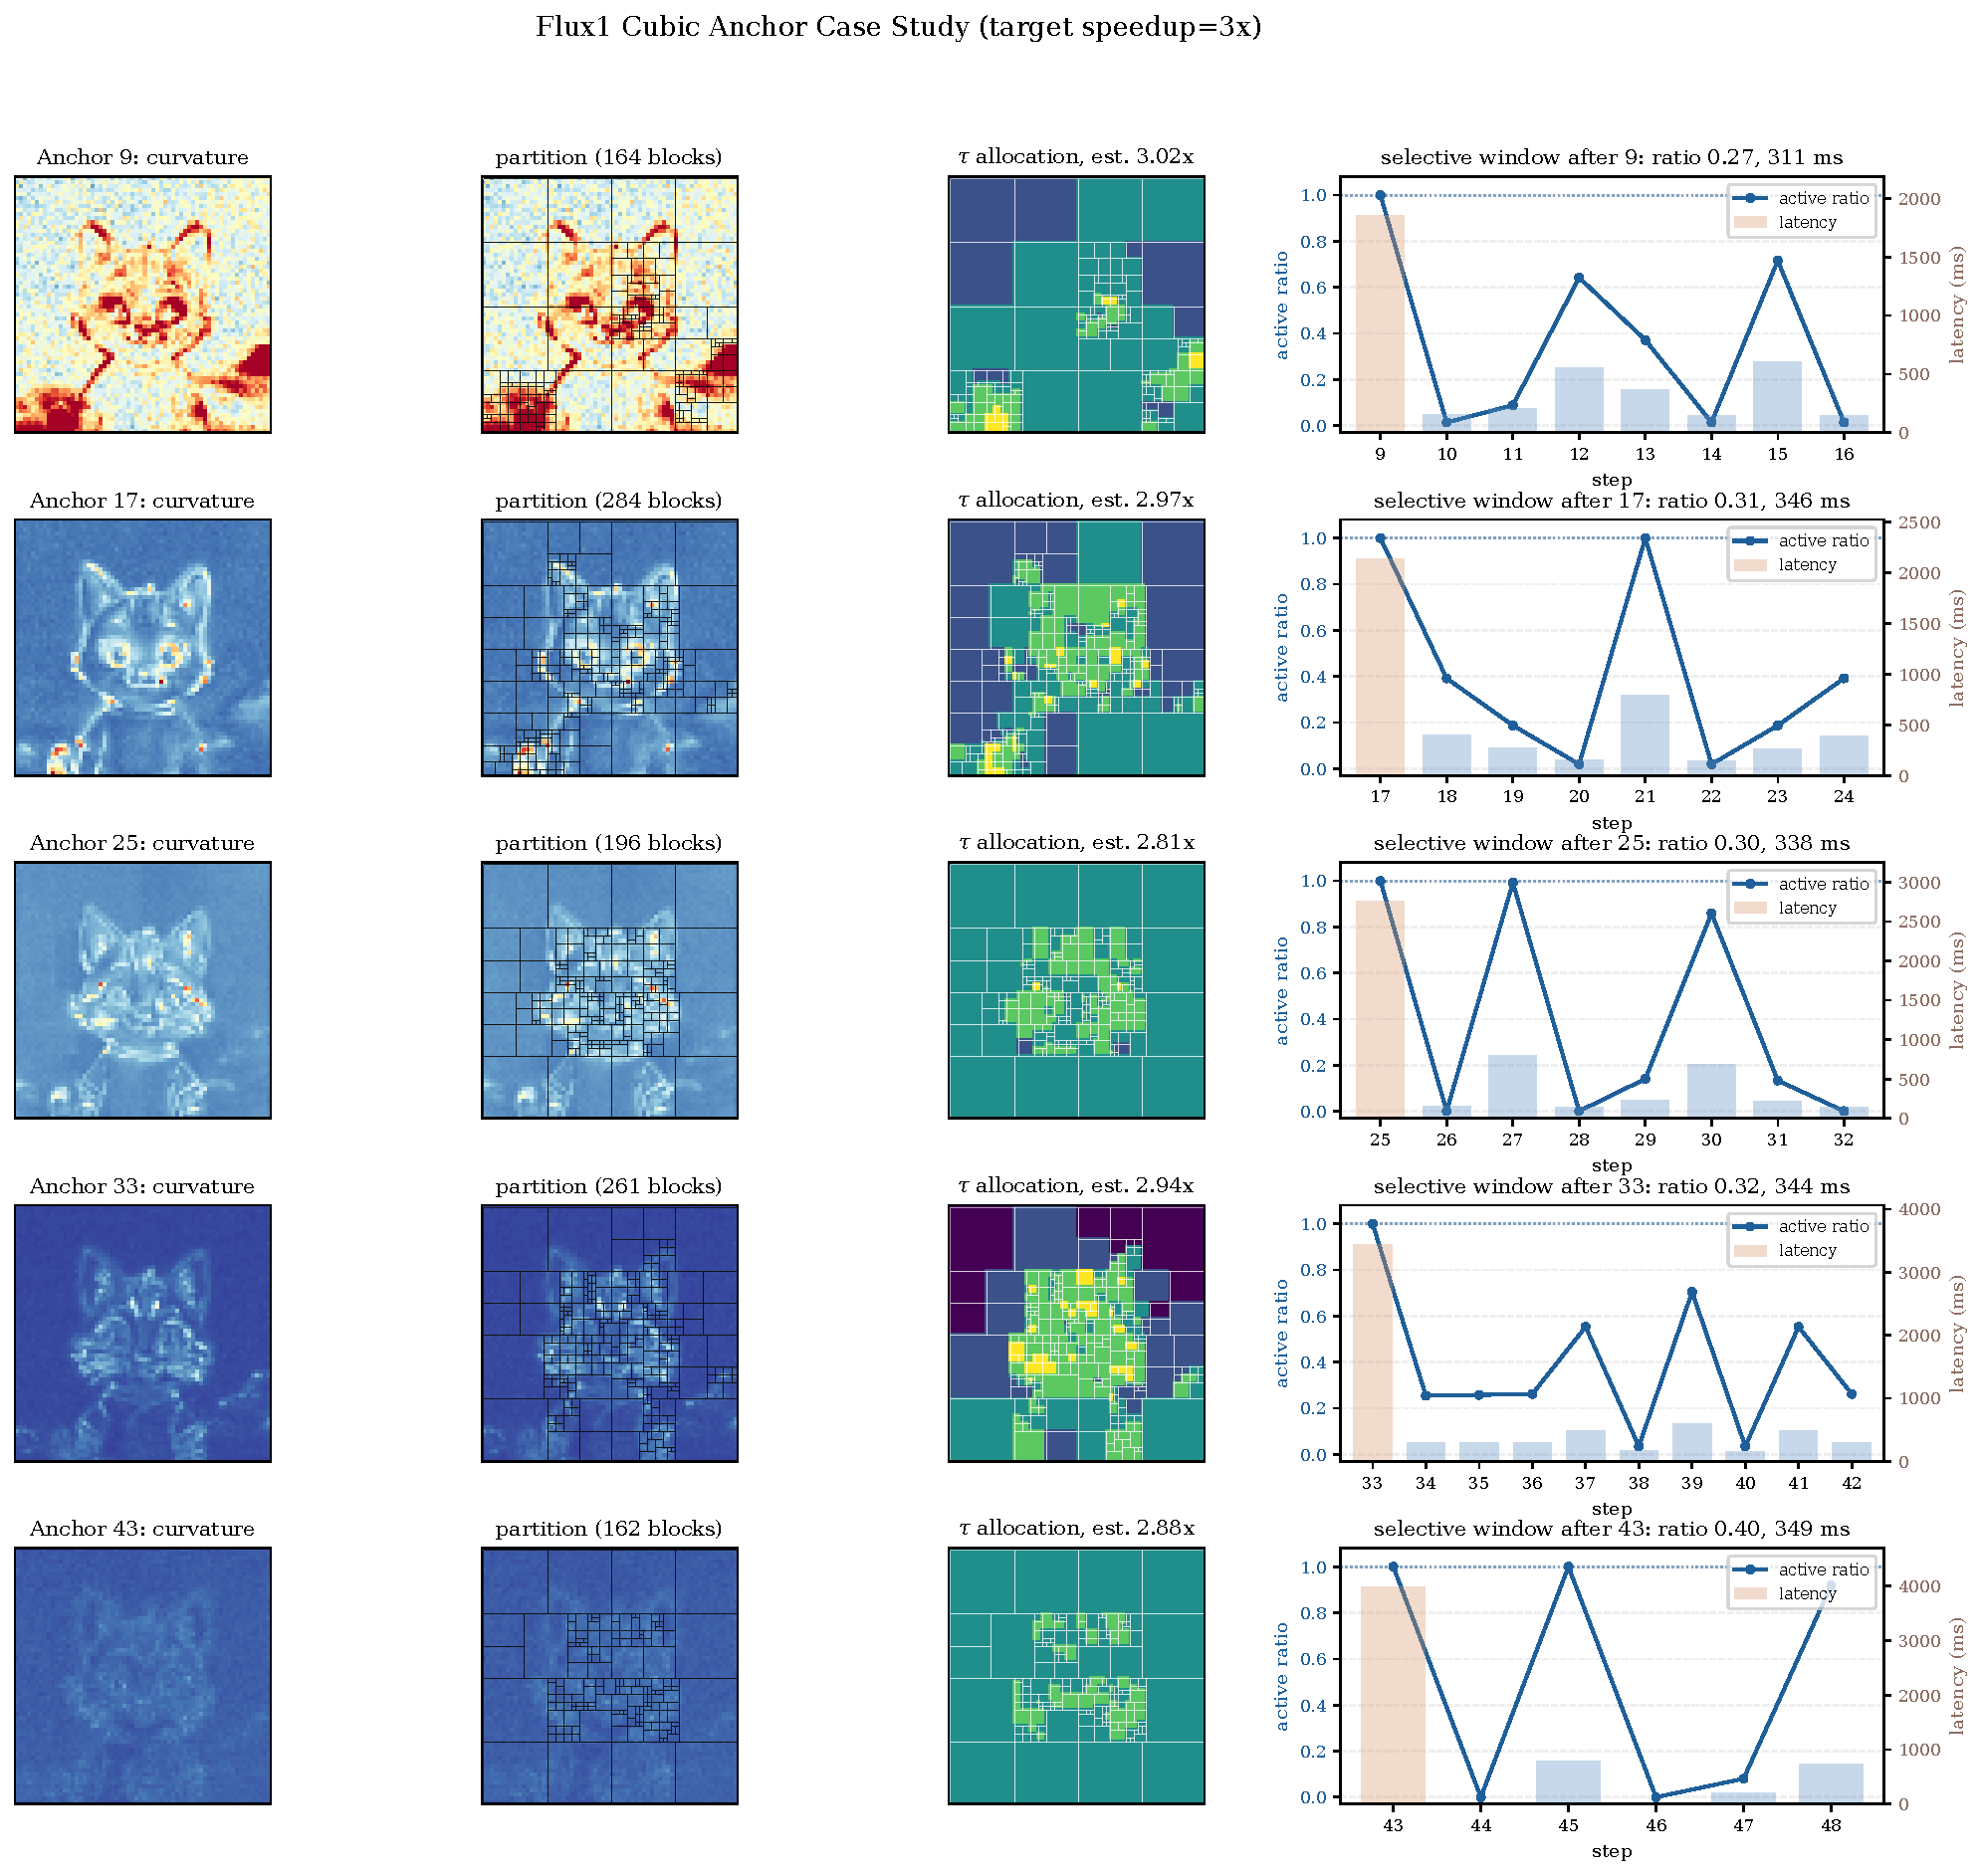
\includegraphics[width=\linewidth]{figure/casestudy.pdf}
    \caption{\cubic case study on Flux.1 with target speedup $3\times$.}
    \label{fig:case_study}
\end{figure}


\newpage
\section{Detailed Results of \cubic Evaluation}
\label{app:detail_result}
We report the detailed parameter settings and performance of \cubic in Table~\ref{tab:detail}. For completeness, Table~\ref{tab:detail_baseline} provides the corresponding configurations and results of other baseline methods.

\begin{table*}[h]
\centering
\caption{Parameters setting and performance of \cubic }
\label{tab:detail}´
\resizebox{0.7\textwidth}{!}{
\begin{tabular}{l c c c c c c}
\toprule
\small
\textbf{Model}
& $\boldsymbol{\rho}$
& $\mathrm{Speedup}\uparrow$
& $\mathrm{PSNR}\uparrow$
& $\mathrm{SSIM}\uparrow$
& $\mathrm{LPIPS}\downarrow$
& $\mathrm{FID/FVD}\downarrow$ \\
\midrule

% ===== Flux-1 =====
\multirow{5}{*}{Flux-1}
& 2  & 1.38$\times$ & 32.03 & 0.9445 & 0.0409 & 12.51 \\
& 4  & 1.89$\times$ & 27.78 & 0.8998 & 0.0946 & 27.81 \\
& 6  & 2.22$\times$ & 26.04 & 0.8691 & 0.1299 & 37.14 \\
& 8  & 2.40$\times$ & 25.14 & 0.8457 & 0.1730 & 47.32 \\
& 10 & 2.51$\times$ & 24.45 & 0.8282 & 0.1964 & 52.82 \\
\midrule

% ===== FireRed =====
\multirow{5}{*}{FireRed}
& 2  & 1.76$\times$ & 33.85 & 0.9711 & 0.0268 & 10.91 \\
& 4  & 2.14$\times$ & 30.67 & 0.9538 & 0.0468 & 18.55 \\
& 6  & 2.23$\times$ & 28.74 & 0.9310 & 0.0769 & 27.15 \\
& 8  & 2.33$\times$ & 27.81 & 0.9201 & 0.0907 & 32.18 \\
& 10 & 2.50$\times$ & 27.06 & 0.9080 & 0.1059 & 38.35 \\
\midrule

% ===== Wan-1.3B =====
\multirow{5}{*}{Wan-1.3B}
& 2  & 1.63$\times$ & 32.76 & 0.9481 & 0.0317 & 7.912 \\
& 4  & 2.30$\times$ & 27.99 & 0.8990 & 0.0728 & 21.14 \\
& 6  & 2.72$\times$ & 26.39 & 0.8740 & 0.0986 & 31.76 \\
& 8  & 3.04$\times$ & 25.50 & 0.8501 & 0.1236 & 45.08 \\
& 10 & 3.23$\times$ & 24.65 & 0.8284 & 0.1437 & 62.48 \\

\bottomrule
\end{tabular}
}
\end{table*}

\begin{table*}[h]
\centering
\caption{Parameters setting and performance of baselines. }
\label{tab:detail_baseline}
\resizebox{0.7\textwidth}{!}{
\begin{tabular}{l l c c c c c}
\toprule
\textbf{Model} & \textbf{Method}
& $\mathrm{Speedup}\uparrow$
& $\mathrm{PSNR}\uparrow$
& $\mathrm{SSIM}\uparrow$
& $\mathrm{LPIPS}\downarrow$
& $\mathrm{FID/FVD}\downarrow$ \\
\midrule

\multirow{12}{*}{\textbf{Flux-1}}
& ToCa(4)         & 1.69$\times$ & 20.34 & 0.7647 & 0.2414 & 61.97 \\
& ToCa(5)         & 1.81$\times$ & 19.68 & 0.7493 & 0.2726 & 70.76\\
& ToCa(6)         & 1.93$\times$ & 18.88 & 0.7094 & 0.3164 & 78.10 \\
& TeaCache(0.25)  & 1.86$\times$ & 22.88 & 0.8514 & 0.1490 & 45.87 \\
& TeaCache(0.4)   & 2.52$\times$ & 19.66 & 0.7720 & 0.2481 & 66.04 \\
& TeaCache(0.6)   & 3.31$\times$ & 17.66 & 0.7279 & 0.3155 & 89.86 \\
& TaylorSeer(N2)  & 1.70$\times$ & 26.29 & 0.8920 & 0.0994 & 26.80 \\
& TaylorSeer(N3)  & 2.25$\times$ & 21.42 & 0.8180 & 0.1796 & 47.53 \\
& TaylorSeer(N4)  & 2.66$\times$ & 19.27 & 0.7606 & 0.2497 & 63.59 \\
& PAB(4)          & 1.62$\times$ & 22.88 & 0.8373 & 0.1613 & 47.83 \\
& PAB(8)          & 1.81$\times$ & 20.37 & 0.7702 & 0.2574 & 77.37 \\
& PAB(12)         & 1.90$\times$ & 19.47 & 0.7344 & 0.3293 & 106.65 \\
\midrule

\multirow{13}{*}{\textbf{FireRed}}
& ToCa(3)     & 1.50$\times$ & 24.17 & 0.8736 & 0.1103 & 49.84 \\
& ToCa(4)     & 1.76$\times$ & 22.57 & 0.8367 & 0.1471 & 62.58 \\
& ToCa(5)     & 1.95$\times$ & 21.09 & 0.7884 & 0.1779 & 67.25 \\
& TeaCache(0.1)   & 1.51$\times$ & 27.49 & 0.9363 & 0.0562 & 25.55 \\
& TeaCache(0.15)  & 2.04$\times$ & 25.65 & 0.9183 & 0.0758 & 31.00 \\
& TeaCache(0.2)   & 2.31$\times$ & 23.80 & 0.8955 & 0.0995 & 41.03 \\
& TaylorSeer(N2)  & 1.86$\times$ & 25.12 & 0.9102 & 0.0837 & 33.70 \\
& TaylorSeer(N3)  & 2.64$\times$ & 21.17 & 0.8356 & 0.1498 & 50.38 \\
& TaylorSeer(N4)  & 3.35$\times$ & 18.96 & 0.7774 & 0.1987 & 64.84 \\
& PAB(6)          & 1.61$\times$ & 25.82 & 0.9112 & 0.0731 & 33.92 \\
& PAB(8)          & 1.65$\times$ & 24.39 & 0.8888 & 0.0929 & 39.41 \\
& PAB(12)         & 1.68$\times$ & 22.45 & 0.8530 & 0.1312 & 54.07 \\
& PAB(16)         & 1.72$\times$ & 20.87 & 0.9198 & 0.1799 & 67.82 \\
\midrule

\multirow{12}{*}{\textbf{Wan1.3B}}
& ToCa(242)        & 1.69$\times$ & 19.60 & 0.7486 & 0.2273 & 78.95 \\
& ToCa(333)        & 2.21$\times$ & 20.66 & 0.7684 & 0.1949 & 66.02 \\
& ToCa(363)        & 2.31$\times$ & 19.19 & 0.7383 & 0.2405 & 84.04 \\
& TeaCache(0.05)   & 1.65$\times$ & 30.27 & 0.9270 & 0.0454 & 11.72 \\
& TeaCache(0.07)   & 1.75$\times$ & 26.38 & 0.8684 & 0.0933 & 24.85 \\
& TeaCache(0.08)   & 2.15$\times$ & 24.51 & 0.8405 & 0.1206 & 35.26 \\
& TaylorSeer(N2)   & 1.91$\times$ & 18.29 & 0.7225 & 0.2504 & 94.59 \\
& TaylorSeer(N3)   & 2.59$\times$ & 15.80 & 0.6410 & 0.3521 & 137.06 \\
& TaylorSeer(N4)   & 3.19$\times$ & 14.04 & 0.5837 & 0.4406 & 181.41 \\
& PAB(2,5)         & 1.67$\times$ & 24.06 & 0.8370 & 0.1212 & 36.82 \\
& PAB(4,5)         & 2.17$\times$ & 22.83 & 0.8127 & 0.1530 & 52.37 \\
& PAB(6,6)         & 2.50$\times$ & 22.36 & 0.8000 & 0.1670 & 57.78 \\
\bottomrule
\end{tabular}
}
\end{table*}

\newpage

\section{Visualization of \cubic}
\label{app_vis}
We provide visualization comparison between original video generation and \cubic on Flux-1, FireRed and Wan 2.1. We evaluate \cubic on Text-to-Image generation, Image Editing, and Text-to-Video generation using the default resolution of each model. Results demonstrates \cubic can preserve high pixel-level fidelity, achieving similar generation quality compared with the original generation.
\begin{figure*}[!h]
    \centering
    \includegraphics[width=\textwidth]{figure/flux_ori_cubic_comparison.pdf}
    \caption{Flux visualization comparison between original images (top) and \cubic results (bottom)}
    \label{fig:flux_visual}
\end{figure*}

\begin{figure*}[!h]
    \centering
    \includegraphics[width=\textwidth]{figure/firered_ori_cubic_comparison.pdf}
    \caption{FireRed visualization comparison between original images (top) and \cubic results (bottom)}
    \label{fig:firered_visual}
\end{figure*}

\begin{figure*}[!h]
    \centering
    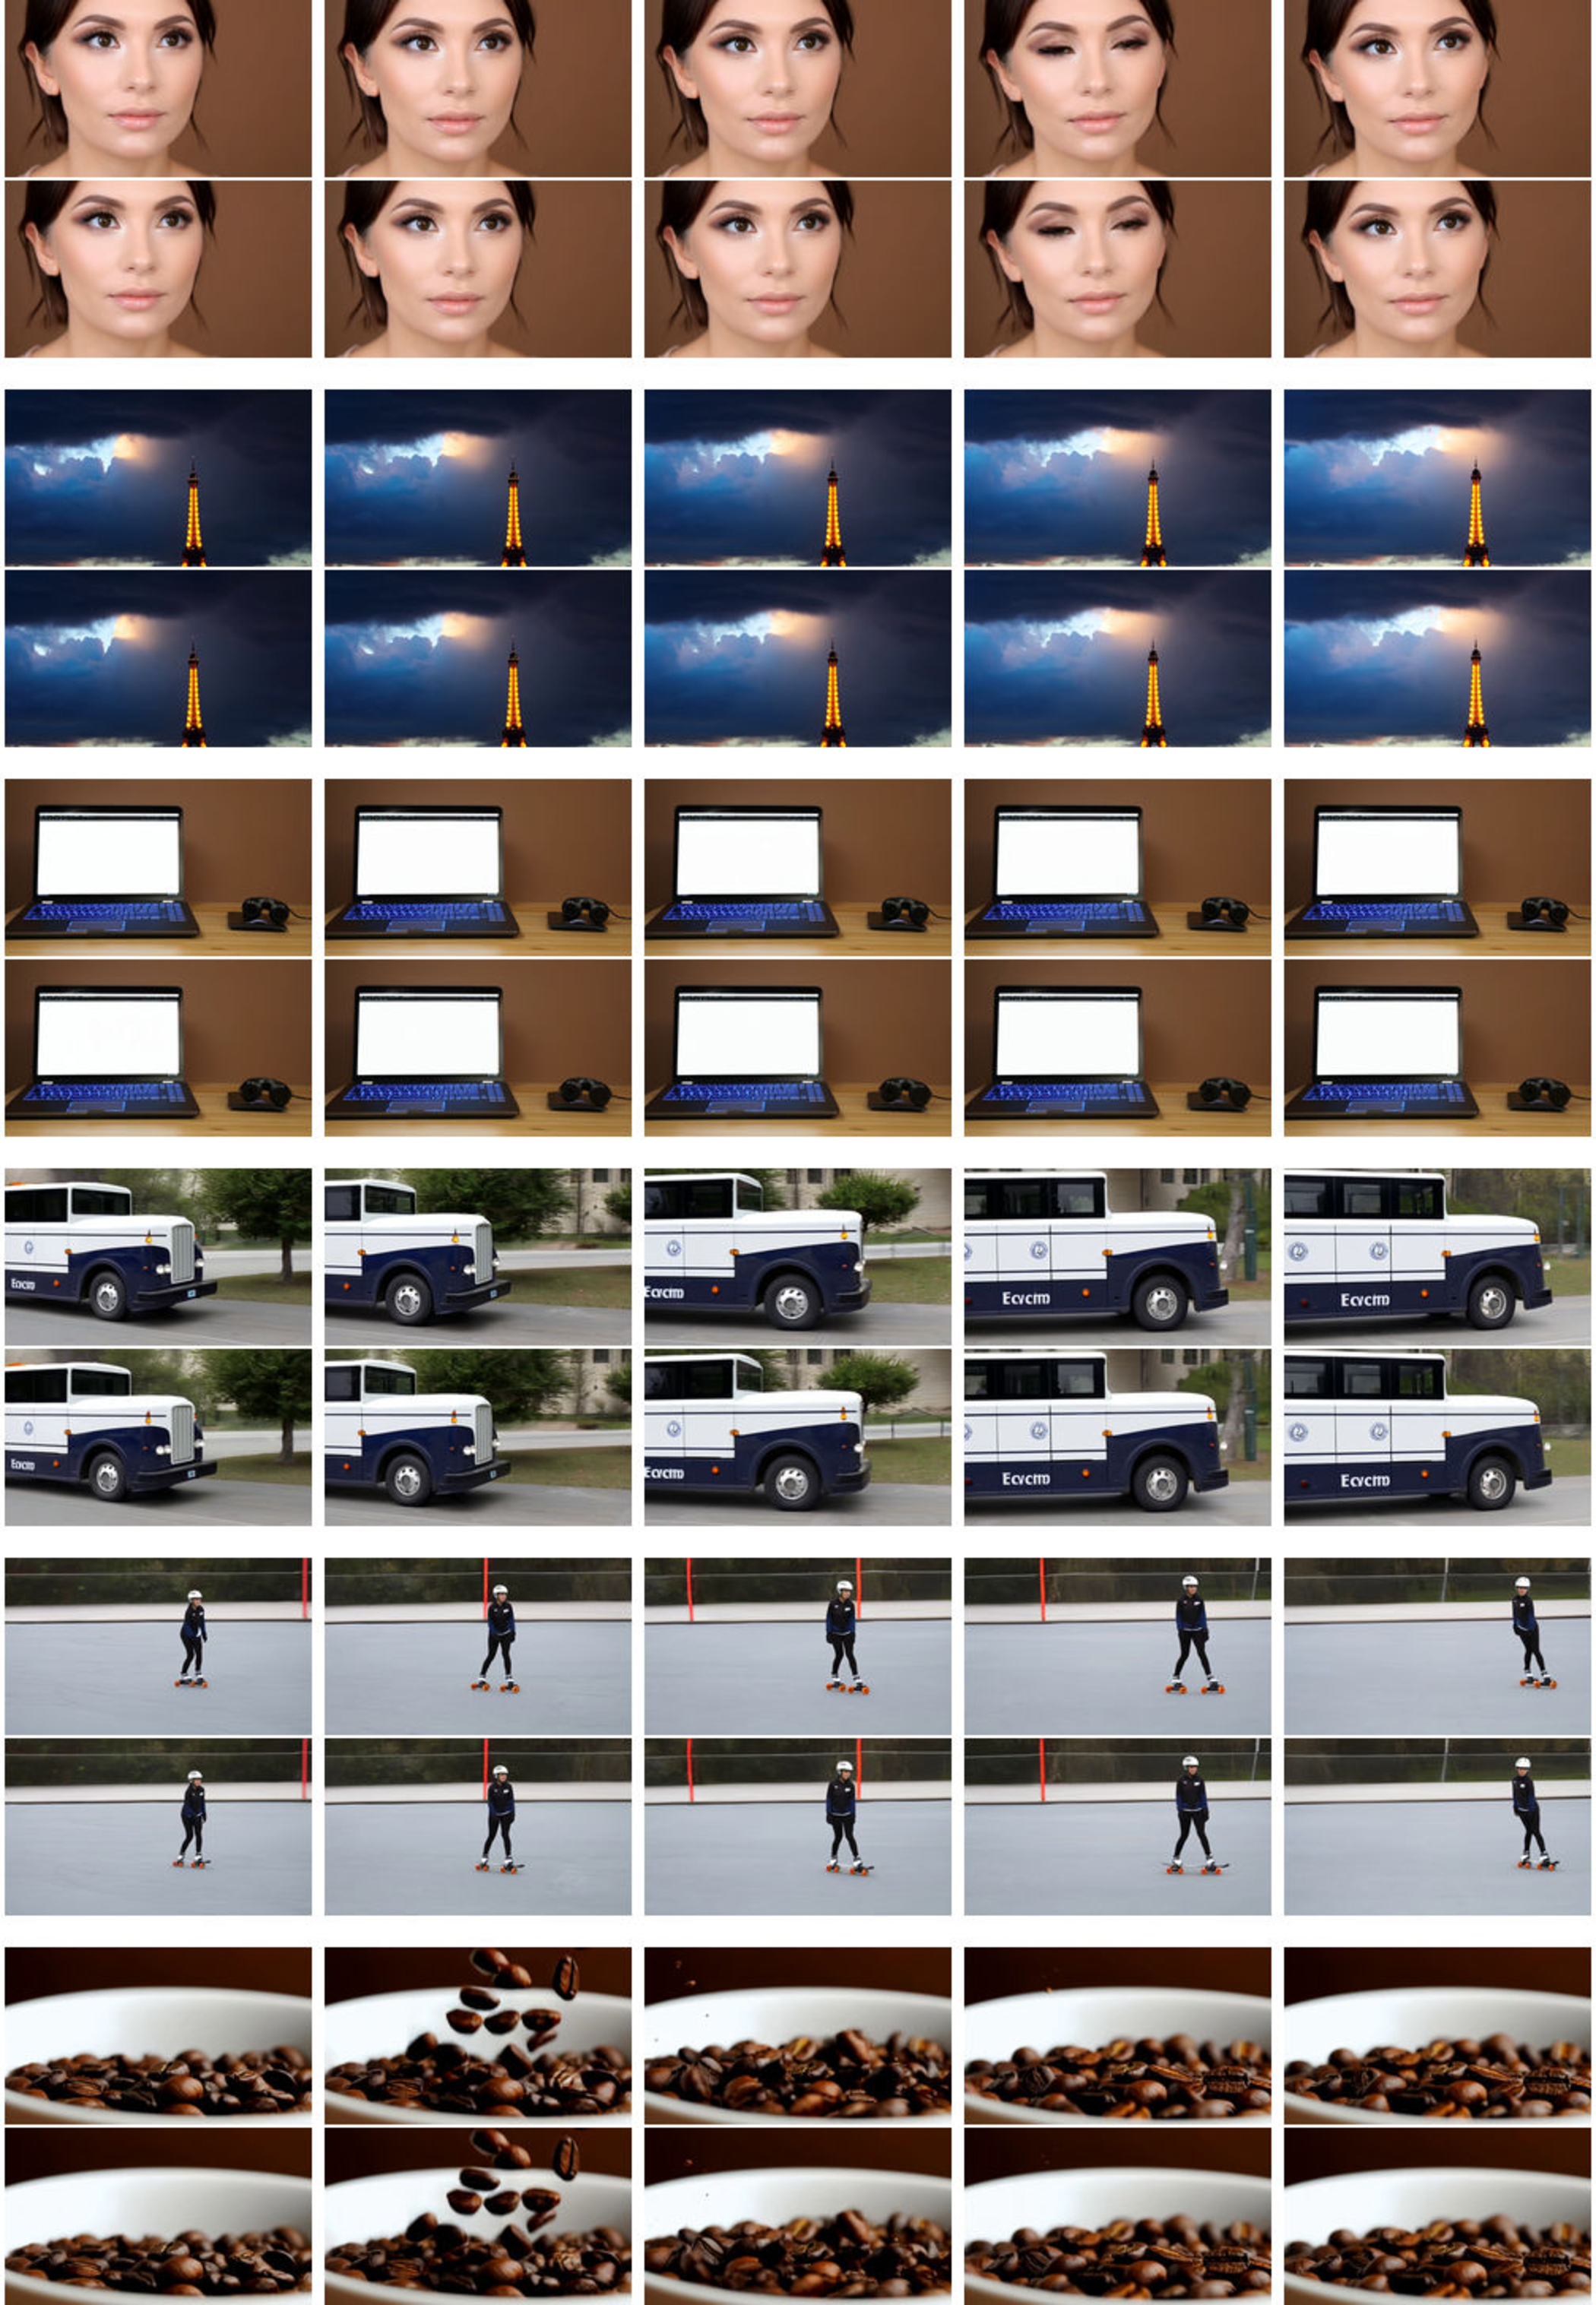
\includegraphics[width=\textwidth]{figure/wan_ori_cubic_video_comparison.pdf}
    \caption{Wan 1.3B visualization comparison between original vedios (top) and \cubic results (bottom)}
    \label{fig:wan_visual}
\end{figure*}

\clearpage
\section*{NeurIPS Paper Checklist}

% %%% BEGIN INSTRUCTIONS %%%
% The checklist is designed to encourage best practices for responsible machine learning research, addressing issues of reproducibility, transparency, research ethics, and societal impact. Do not remove the checklist: {\bf The papers not including the checklist will be desk rejected.} The checklist should follow the references and follow the (optional) supplemental material.  The checklist does NOT count towards the page
% limit. 

% Please read the checklist guidelines carefully for information on how to answer these questions. For each question in the checklist:
% \begin{itemize}
%     \item You should answer \answerYes{}, \answerNo{}, or \answerNA{}.
%     \item \answerNA{} means either that the question is Not Applicable for that particular paper or the relevant information is Not Available.
%     \item Please provide a short (1--2 sentence) justification right after your answer (even for \answerNA). 
%    % \item {\bf The papers not including the checklist will be desk rejected.}
% \end{itemize}

% {\bf The checklist answers are an integral part of your paper submission.} They are visible to the reviewers, area chairs, senior area chairs, and ethics reviewers. You will also be asked to include it (after eventual revisions) with the final version of your paper, and its final version will be published with the paper.

% The reviewers of your paper will be asked to use the checklist as one of the factors in their evaluation. While \answerYes{} is generally preferable to \answerNo{}, it is perfectly acceptable to answer \answerNo{} provided a proper justification is given (e.g., error bars are not reported because it would be too computationally expensive'' or ``we were unable to find the license for the dataset we used''). In general, answering \answerNo{} or \answerNA{} is not grounds for rejection. While the questions are phrased in a binary way, we acknowledge that the true answer is often more nuanced, so please just use your best judgment and write a justification to elaborate. All supporting evidence can appear either in the main paper or the supplemental material, provided in appendix. If you answer \answerYes{} to a question, in the justification please point to the section(s) where related material for the question can be found.

% IMPORTANT, please:
% \begin{itemize}
%     \item {\bf Delete this instruction block, but keep the section heading ``NeurIPS Paper Checklist"},
%     \item  {\bf Keep the checklist subsection headings, questions/answers and guidelines below.}
%     \item {\bf Do not modify the questions and only use the provided macros for your answers}.
% \end{itemize} 
 

% %%% END INSTRUCTIONS %%%


\begin{enumerate}

\item {\bf Claims}
    \item[] Question: Do the main claims made in the abstract and introduction accurately reflect the paper's contributions and scope?
    \item[] Answer: \answerYes{} % Replace by \answerYes{}, \answerNo{}, or \answerNA{}.
    \item[] Justification: Abstract and section~\ref{sec:intro}  reflect the paper's contributions and scope. 
    \item[] Guidelines:
    \begin{itemize}
        \item The answer \answerNA{} means that the abstract and introduction do not include the claims made in the paper.
        \item The abstract and/or introduction should clearly state the claims made, including the contributions made in the paper and important assumptions and limitations. A \answerNo{} or \answerNA{} answer to this question will not be perceived well by the reviewers. 
        \item The claims made should match theoretical and experimental results, and reflect how much the results can be expected to generalize to other settings. 
        \item It is fine to include aspirational goals as motivation as long as it is clear that these goals are not attained by the paper. 
    \end{itemize}

\item {\bf Limitations}
    \item[] Question: Does the paper discuss the limitations of the work performed by the authors?
    \item[] Answer: \answerYes{} % Replace by \answerYes{}, \answerNo{}, or \answerNA{}.
    \item[] Justification: Sec.~\ref{sec:conclusion} discuss the limitations of \cubic.
    \item[] Guidelines:
    \begin{itemize}
        \item The answer \answerNA{} means that the paper has no limitation while the answer \answerNo{} means that the paper has limitations, but those are not discussed in the paper. 
        \item The authors are encouraged to create a separate ``Limitations'' section in their paper.
        \item The paper should point out any strong assumptions and how robust the results are to violations of these assumptions (e.g., independence assumptions, noiseless settings, model well-specification, asymptotic approximations only holding locally). The authors should reflect on how these assumptions might be violated in practice and what the implications would be.
        \item The authors should reflect on the scope of the claims made, e.g., if the approach was only tested on a few datasets or with a few runs. In general, empirical results often depend on implicit assumptions, which should be articulated.
        \item The authors should reflect on the factors that influence the performance of the approach. For example, a facial recognition algorithm may perform poorly when image resolution is low or images are taken in low lighting. Or a speech-to-text system might not be used reliably to provide closed captions for online lectures because it fails to handle technical jargon.
        \item The authors should discuss the computational efficiency of the proposed algorithms and how they scale with dataset size.
        \item If applicable, the authors should discuss possible limitations of their approach to address problems of privacy and fairness.
        \item While the authors might fear that complete honesty about limitations might be used by reviewers as grounds for rejection, a worse outcome might be that reviewers discover limitations that aren't acknowledged in the paper. The authors should use their best judgment and recognize that individual actions in favor of transparency play an important role in developing norms that preserve the integrity of the community. Reviewers will be specifically instructed to not penalize honesty concerning limitations.
    \end{itemize}

\item {\bf Theory assumptions and proofs}
    \item[] Question: For each theoretical result, does the paper provide the full set of assumptions and a complete (and correct) proof?
    \item[] Answer: \answerYes{} % Replace by \answerYes{}, \answerNo{}, or \answerNA{}.
    \item[] Justification: Section~\ref{sec:method} and Appendix~\ref{app:cubic_theory} provide rigorous theoretical derivations and proofs.

    \item[] Guidelines:
    \begin{itemize}
        \item The answer \answerNA{} means that the paper does not include theoretical results. 
        \item All the theorems, formulas, and proofs in the paper should be numbered and cross-referenced.
        \item All assumptions should be clearly stated or referenced in the statement of any theorems.
        \item The proofs can either appear in the main paper or the supplemental material, but if they appear in the supplemental material, the authors are encouraged to provide a short proof sketch to provide intuition. 
        \item Inversely, any informal proof provided in the core of the paper should be complemented by formal proofs provided in appendix or supplemental material.
        \item Theorems and Lemmas that the proof relies upon should be properly referenced. 
    \end{itemize}

    \item {\bf Experimental result reproducibility}
    \item[] Question: Does the paper fully disclose all the information needed to reproduce the main experimental results of the paper to the extent that it affects the main claims and/or conclusions of the paper (regardless of whether the code and data are provided or not)?
    \item[] Answer: \answerYes{} % Replace by \answerYes{}, \answerNo{}, or \answerNA{}.
    \item[] Justification: We provide a detailed implementation of \cubic. All experiments use publicly available datasets and models,
ensuring reproducibility. 
    \item[] Guidelines:
    \begin{itemize}
        \item The answer \answerNA{} means that the paper does not include experiments.
        \item If the paper includes experiments, a \answerNo{} answer to this question will not be perceived well by the reviewers: Making the paper reproducible is important, regardless of whether the code and data are provided or not.
        \item If the contribution is a dataset and\slash or model, the authors should describe the steps taken to make their results reproducible or verifiable. 
        \item Depending on the contribution, reproducibility can be accomplished in various ways. For example, if the contribution is a novel architecture, describing the architecture fully might suffice, or if the contribution is a specific model and empirical evaluation, it may be necessary to either make it possible for others to replicate the model with the same dataset, or provide access to the model. In general. releasing code and data is often one good way to accomplish this, but reproducibility can also be provided via detailed instructions for how to replicate the results, access to a hosted model (e.g., in the case of a large language model), releasing of a model checkpoint, or other means that are appropriate to the research performed.
        \item While NeurIPS does not require releasing code, the conference does require all submissions to provide some reasonable avenue for reproducibility, which may depend on the nature of the contribution. For example
        \begin{enumerate}
            \item If the contribution is primarily a new algorithm, the paper should make it clear how to reproduce that algorithm.
            \item If the contribution is primarily a new model architecture, the paper should describe the architecture clearly and fully.
            \item If the contribution is a new model (e.g., a large language model), then there should either be a way to access this model for reproducing the results or a way to reproduce the model (e.g., with an open-source dataset or instructions for how to construct the dataset).
            \item We recognize that reproducibility may be tricky in some cases, in which case authors are welcome to describe the particular way they provide for reproducibility. In the case of closed-source models, it may be that access to the model is limited in some way (e.g., to registered users), but it should be possible for other researchers to have some path to reproducing or verifying the results.
        \end{enumerate}
    \end{itemize}


\item {\bf Open access to data and code}
    \item[] Question: Does the paper provide open access to the data and code, with sufficient instructions to faithfully reproduce the main experimental results, as described in supplemental material?
    \item[] Answer: \answerNo{} % Replace by \answerYes{}, \answerNo{}, or \answerNA{}.
    \item[] Justification: If the paper is accepted or released on arXiv, we will open-source the implementation and provide detailed instructions for reproducing the main experimental results.
    \item[] Guidelines:
    \begin{itemize}
        \item The answer \answerNA{} means that paper does not include experiments requiring code.
        \item Please see the NeurIPS code and data submission guidelines (\url{https://neurips.cc/public/guides/CodeSubmissionPolicy}) for more details.
        \item While we encourage the release of code and data, we understand that this might not be possible, so \answerNo{} is an acceptable answer. Papers cannot be rejected simply for not including code, unless this is central to the contribution (e.g., for a new open-source benchmark).
        \item The instructions should contain the exact command and environment needed to run to reproduce the results. See the NeurIPS code and data submission guidelines (\url{https://neurips.cc/public/guides/CodeSubmissionPolicy}) for more details.
        \item The authors should provide instructions on data access and preparation, including how to access the raw data, preprocessed data, intermediate data, and generated data, etc.
        \item The authors should provide scripts to reproduce all experimental results for the new proposed method and baselines. If only a subset of experiments are reproducible, they should state which ones are omitted from the script and why.
        \item At submission time, to preserve anonymity, the authors should release anonymized versions (if applicable).
        \item Providing as much information as possible in supplemental material (appended to the paper) is recommended, but including URLs to data and code is permitted.
    \end{itemize}


\item {\bf Experimental setting/details}
    \item[] Question: Does the paper specify all the training and test details (e.g., data splits, hyperparameters, how they were chosen, type of optimizer) necessary to understand the results?
    \item[] Answer: \answerYes{} % Replace by \answerYes{}, \answerNo{}, or \answerNA{}.
    \item[] Justification: Section~\ref{sec:method} and Appendix~\ref{app:detail_result} outlines the experimental setup used for all results. 
    \item[] Guidelines:
    \begin{itemize}
        \item The answer \answerNA{} means that the paper does not include experiments.
        \item The experimental setting should be presented in the core of the paper to a level of detail that is necessary to appreciate the results and make sense of them.
        \item The full details can be provided either with the code, in appendix, or as supplemental material.
    \end{itemize}

\item {\bf Experiment statistical significance}
    \item[] Question: Does the paper report error bars suitably and correctly defined or other appropriate information about the statistical significance of the experiments?
    \item[] Answer: \answerYes{} % Replace by \answerYes{}, \answerNo{}, or \answerNA{}.
    \item[] Justification: We report the mean and standard deviation of inference
time across as shown in Table~\ref{tab:results}.
    \item[] Guidelines:
    \begin{itemize}
        \item The answer \answerNA{} means that the paper does not include experiments.
        \item The authors should answer \answerYes{} if the results are accompanied by error bars, confidence intervals, or statistical significance tests, at least for the experiments that support the main claims of the paper.
        \item The factors of variability that the error bars are capturing should be clearly stated (for example, train/test split, initialization, random drawing of some parameter, or overall run with given experimental conditions).
        \item The method for calculating the error bars should be explained (closed form formula, call to a library function, bootstrap, etc.)
        \item The assumptions made should be given (e.g., Normally distributed errors).
        \item It should be clear whether the error bar is the standard deviation or the standard error of the mean.
        \item It is OK to report 1-sigma error bars, but one should state it. The authors should preferably report a 2-sigma error bar than state that they have a 96\% CI, if the hypothesis of Normality of errors is not verified.
        \item For asymmetric distributions, the authors should be careful not to show in tables or figures symmetric error bars that would yield results that are out of range (e.g., negative error rates).
        \item If error bars are reported in tables or plots, the authors should explain in the text how they were calculated and reference the corresponding figures or tables in the text.
    \end{itemize}

\item {\bf Experiments compute resources}
    \item[] Question: For each experiment, does the paper provide sufficient information on the computer resources (type of compute workers, memory, time of execution) needed to reproduce the experiments?
    \item[] Answer: \answerYes{} % Replace by \answerYes{}, \answerNo{}, or \answerNA{}.
    \item[] Justification: We present the resources used for experiments in section~\ref{sec:Implementation}.
    \item[] Guidelines:
    \begin{itemize}
        \item The answer \answerNA{} means that the paper does not include experiments.
        \item The paper should indicate the type of compute workers CPU or GPU, internal cluster, or cloud provider, including relevant memory and storage.
        \item The paper should provide the amount of compute required for each of the individual experimental runs as well as estimate the total compute. 
        \item The paper should disclose whether the full research project required more compute than the experiments reported in the paper (e.g., preliminary or failed experiments that didn't make it into the paper). 
    \end{itemize}
    
\item {\bf Code of ethics}
    \item[] Question: Does the research conducted in the paper conform, in every respect, with the NeurIPS Code of Ethics \url{https://neurips.cc/public/EthicsGuidelines}?
    \item[] Answer: \answerYes{} % Replace by \answerYes{}, \answerNo{}, or \answerNA{}.
    \item[] Justification: This paper conforms with the NeurIPS code of ethics in every respect.
    \item[] Guidelines:
    \begin{itemize}
        \item The answer \answerNA{} means that the authors have not reviewed the NeurIPS Code of Ethics.
        \item If the authors answer \answerNo, they should explain the special circumstances that require a deviation from the Code of Ethics.
        \item The authors should make sure to preserve anonymity (e.g., if there is a special consideration due to laws or regulations in their jurisdiction).
    \end{itemize}


\item {\bf Broader impacts}
    \item[] Question: Does the paper discuss both potential positive societal impacts and negative societal impacts of the work performed?
    \item[] Answer: \answerNA{} % Replace by \answerYes{}, \answerNo{}, or \answerNA{}.
    \item[] Justification: This paper studies a training-free caching strategy for accelerating Flow Matching inference. The method does not introduce new data, new model capabilities, or application-specific deployment scenarios; it only modifies the inference computation schedule to reduce latency. Therefore, potential societal impacts are indirect and primarily depend on the underlying models and their use cases rather than on the proposed acceleration technique itself. 
    \item[] Guidelines:
    \begin{itemize}
        \item The answer \answerNA{} means that there is no societal impact of the work performed.
        \item If the authors answer \answerNA{} or \answerNo, they should explain why their work has no societal impact or why the paper does not address societal impact.
        \item Examples of negative societal impacts include potential malicious or unintended uses (e.g., disinformation, generating fake profiles, surveillance), fairness considerations (e.g., deployment of technologies that could make decisions that unfairly impact specific groups), privacy considerations, and security considerations.
        \item The conference expects that many papers will be foundational research and not tied to particular applications, let alone deployments. However, if there is a direct path to any negative applications, the authors should point it out. For example, it is legitimate to point out that an improvement in the quality of generative models could be used to generate Deepfakes for disinformation. On the other hand, it is not needed to point out that a generic algorithm for optimizing neural networks could enable people to train models that generate Deepfakes faster.
        \item The authors should consider possible harms that could arise when the technology is being used as intended and functioning correctly, harms that could arise when the technology is being used as intended but gives incorrect results, and harms following from (intentional or unintentional) misuse of the technology.
        \item If there are negative societal impacts, the authors could also discuss possible mitigation strategies (e.g., gated release of models, providing defenses in addition to attacks, mechanisms for monitoring misuse, mechanisms to monitor how a system learns from feedback over time, improving the efficiency and accessibility of ML).
    \end{itemize}
    
\item {\bf Safeguards}
    \item[] Question: Does the paper describe safeguards that have been put in place for responsible release of data or models that have a high risk for misuse (e.g., pre-trained language models, image generators, or scraped datasets)?
    \item[] Answer: \answerNA{} % Replace by \answerYes{}, \answerNo{}, or \answerNA{}.
    \item[] Justification: This paper does not introduce or release new high-risk datasets or generative models.
    \item[] Guidelines:
    \begin{itemize}
        \item The answer \answerNA{} means that the paper poses no such risks.
        \item Released models that have a high risk for misuse or dual-use should be released with necessary safeguards to allow for controlled use of the model, for example by requiring that users adhere to usage guidelines or restrictions to access the model or implementing safety filters. 
        \item Datasets that have been scraped from the Internet could pose safety risks. The authors should describe how they avoided releasing unsafe images.
        \item We recognize that providing effective safeguards is challenging, and many papers do not require this, but we encourage authors to take this into account and make a best faith effort.
    \end{itemize}

\item {\bf Licenses for existing assets}
    \item[] Question: Are the creators or original owners of assets (e.g., code, data, models), used in the paper, properly credited and are the license and terms of use explicitly mentioned and properly respected?
    \item[] Answer: \answerYes{} % Replace by \answerYes{}, \answerNo{}, or \answerNA{}.
    \item[] Justification: All the models and datasets are properly cited.
    \item[] Guidelines:
    \begin{itemize}
        \item The answer \answerNA{} means that the paper does not use existing assets.
        \item The authors should cite the original paper that produced the code package or dataset.
        \item The authors should state which version of the asset is used and, if possible, include a URL.
        \item The name of the license (e.g., CC-BY 4.0) should be included for each asset.
        \item For scraped data from a particular source (e.g., website), the copyright and terms of service of that source should be provided.
        \item If assets are released, the license, copyright information, and terms of use in the package should be provided. For popular datasets, \url{paperswithcode.com/datasets} has curated licenses for some datasets. Their licensing guide can help determine the license of a dataset.
        \item For existing datasets that are re-packaged, both the original license and the license of the derived asset (if it has changed) should be provided.
        \item If this information is not available online, the authors are encouraged to reach out to the asset's creators.
    \end{itemize}

\item {\bf New assets}
    \item[] Question: Are new assets introduced in the paper well documented and is the documentation provided alongside the assets?
    \item[] Answer: \answerNA{} % Replace by \answerYes{}, \answerNo{}, or \answerNA{}.
    \item[] Justification: This paper does not introduce or release new assets such as datasets, pretrained models, or benchmark suites. 
    \item[] Guidelines:
    \begin{itemize}
        \item The answer \answerNA{} means that the paper does not release new assets.
        \item Researchers should communicate the details of the dataset\slash code\slash model as part of their submissions via structured templates. This includes details about training, license, limitations, etc. 
        \item The paper should discuss whether and how consent was obtained from people whose asset is used.
        \item At submission time, remember to anonymize your assets (if applicable). You can either create an anonymized URL or include an anonymized zip file.
    \end{itemize}

\item {\bf Crowdsourcing and research with human subjects}
    \item[] Question: For crowdsourcing experiments and research with human subjects, does the paper include the full text of instructions given to participants and screenshots, if applicable, as well as details about compensation (if any)? 
    \item[] Answer: \answerNA{} % Replace by \answerYes{}, \answerNo{}, or \answerNA{}.
    \item[] Justification: Paper does not involve crowdsourcing or research with human subjects.
    \item[] Guidelines:
    \begin{itemize}
        \item The answer \answerNA{} means that the paper does not involve crowdsourcing nor research with human subjects.
        \item Including this information in the supplemental material is fine, but if the main contribution of the paper involves human subjects, then as much detail as possible should be included in the main paper. 
        \item According to the NeurIPS Code of Ethics, workers involved in data collection, curation, or other labor should be paid at least the minimum wage in the country of the data collector. 
    \end{itemize}

\item {\bf Institutional review board (IRB) approvals or equivalent for research with human subjects}
    \item[] Question: Does the paper describe potential risks incurred by study participants, whether such risks were disclosed to the subjects, and whether Institutional Review Board (IRB) approvals (or an equivalent approval/review based on the requirements of your country or institution) were obtained?
    \item[] Answer: \answerNA{} % Replace by \answerYes{}, \answerNo{}, or \answerNA{}.
    \item[] Justification: Paper does not involve crowdsourcing or research with human subjects.
    \item[] Guidelines:
    \begin{itemize}
        \item The answer \answerNA{} means that the paper does not involve crowdsourcing nor research with human subjects.
        \item Depending on the country in which research is conducted, IRB approval (or equivalent) may be required for any human subjects research. If you obtained IRB approval, you should clearly state this in the paper. 
        \item We recognize that the procedures for this may vary significantly between institutions and locations, and we expect authors to adhere to the NeurIPS Code of Ethics and the guidelines for their institution. 
        \item For initial submissions, do not include any information that would break anonymity (if applicable), such as the institution conducting the review.
    \end{itemize}

\item {\bf Declaration of LLM usage}
    \item[] Question: Does the paper describe the usage of LLMs if it is an important, original, or non-standard component of the core methods in this research? Note that if the LLM is used only for writing, editing, or formatting purposes and does \emph{not} impact the core methodology, scientific rigor, or originality of the research, declaration is not required.
    %this research? 
    \item[] Answer: \answerNA{} % Replace by \answerYes{}, \answerNo{}, or \answerNA{}.
    \item[] Justification: \cubic does not involve LLMs
    \item[] Guidelines:
    \begin{itemize}
        \item The answer \answerNA{} means that the core method development in this research does not involve LLMs as any important, original, or non-standard components.
        \item Please refer to our LLM policy in the NeurIPS handbook for what should or should not be described.
    \end{itemize}

\end{enumerate}
\end{document}
